% ======================================================================================
% Introduction
% ======================================================================================
\section{\scarc{} verification tests}
\label{SEC_SCARC_verification}

In the following, \scarc{} is subjected to a series of test calculations to demonstrate its suitability as an alternative pressure solver in FDS.  To check whether \scarc{} fundamentally delivers correct results, 
the first step focuses on the analysis of its approximation quality with special view on the handling of multi-mesh decompositions and internal obstructions.
%
For this purpose, a new \scarc{} specific test case {\ct poisson2d} will be presented, which analyzes its various features and variants.
Additionally, \scarc{} is applied to a number of existing verification test cases from FDS.
In order to evaluate the results in a meaningful way, all \scarc{} computations are compared with the respective computations of the other available pressure solvers based on FFT or global $LU$-decomposition. Subsequently, both structured and unstructured discretizations are taken into account and the respective solvers including their short names are summarized below.

\subsection{Summary of solvers applied}

%It has already been explained that only special combinations of discretization types and solvers can be applied. The variants used in the test calculations, including their short names, are listed below.
%
\paragraph{Structured discretizations:} 
In case of a structured discretization, different variants of FFT and structured \scarc{} will be considered.
Due to their structured nature, FFT and \scarc{} are not able to incorporate the right boundary conditions along internal obstructions 
as explained in Section (\ref{SEC_SCARC_discretization_types}). 
Thus, both are embedded in the corrective pressure iteration which applies them several times until the predefined velocity tolerance has been fulfilled, see again Figure \ref{FIG_SCARC_multi_pipe_fft_presite} and Figure \ref{FIG_default_scarc}.
In case of FFT the pressure iteration additionally serves to correct the velocity errors along mesh interfaces. In contrast, \scarc{} doesn't need any further correction there because the inter-mesh transitions of the flow field are consistent by design. 

To analyze the effectiveness of the pressure iteration for a given test case, both FFT and \scarc{} take into account the default and a finer value for the velocity tolerance. Since FFT is basically the default pressure solver in FDS, it does not have to be specified separately.
For \scarc{} the extra specification {\ct SOLVER='SCARC'} must be used in the {\ct \&PRES} name list, see
again Section (\ref{SEC_SCARC_application_notes}).

\begin{itemize}
\item The variants with default velocity tolerance are denoted by \fftdefault{} and \scarcdefault{}. Apart from the basic solver selection, nothing more needs to be specified. The default value for {\ct VELOCITY\_TOLERANCE} is automatically set corresponding to the respective grid width and a default limit of 10 is used for  {\ct MAX\_PRESSURE\_ITERATIONS}. 
\item The variants with finer velocity tolerance are denoted by \ffttight{} and \scarctight{}. The desired value of {\ct VELOCITY\_TOLERANCE} must additionally be specified in the {\ct \&PRES} namelist which is done individually for the different test cases. For both variants the increased setting of {\ct MAX\_PRESSURE\_ITERATIONS=1000} is basically used.
\end{itemize}
%
Both \scarcdefault{} and \scarctight{} are based on a data-parallel global CG-method using an \ols{}-preconditioning by mesh-wise FFT-methods.
In some of the subsequent cases two further generalized variants for \scarc{} will be used. The first variant, \scarctwolevel{}, is also CG-based, but uses a \tls{} preconditioning incorporating an additional coarse grid. The second one, \scarcmultigrid{}, uses a global MG-method instead of the global CG-method and is based on local SSOR-smoothers. Both will only be applied in their default variant, i.e.\ with the related default velocity tolerance.

\paragraph{Unstructured discretizations:} \mbox{} \\[1ex]
In case of an unstructured discretization, FFT can no longer be applied. 
Instead, the alternative pressure solver \uglmat{} is used, which is based on the computation of a global $LU$-decomposition using the optimized parallel {\ct Cluster\_Sparse\_Solver} of the Intel\textsuperscript{\textregistered} MKL library as described in Section (\ref{SEC_SCARC_lu_decomposition}).
Furthermore, \uscarc{} as the unstructured counterpart of \scarc{} will be applied, see Figure \ref{FIG_default_uscarc} again.
To call these solvers the additional settings  {\ct SOLVER='UGLMAT'} or {\ct SOLVER='USCARC'} must be used in the {\ct \&PRES} namelist, respectively.

Both \uglmat{} and \uscarc{} are able to correctly treat mesh interfaces and internal obstructions without additional pressure iteration. Thus, no specification of a velocity tolerance is required and machine accuracy is achieved by design.
Again, \uscarc{} relies on a global CG-method by default. However, due to the unstructured nature of the single sub-grids, the preconditioning can no longer be done by local FFTs. Instead, local $LU$-decompositions are used by default which are based on the optimized serial {\ct PARDISO} solver of the Intel\textsuperscript{\textregistered} MKL Library. 

As mentioned earlier, the local $LU$ decompositions prove to be slower than the local FFTs. Thus,
it may happen that \uscarc{} (which exactly needs one pressure iteration) may be nevertheless slower than a corresponding \scarc{} (if it succeeds to rapidly reach its velocity tolerance in only a few pressure iterations). Optimized strategies to remedy this situation are in work.

\vspace{0.3in}
Now, the crucial question is how well the different structured and unstructured variants are able to preserve the accuracy of the corresponding exact solutions and how good they can be scaled to larger numbers of sub-meshes. To provide a better overview, the solvers including their discretization types and their short names are summarized again in Table \ref{TAB_scarc_overview_pressure_solvers}. 


\begin{table}[h]
\begin{center}
{
\begin{tabular}{|c|c|l|c|c|}
\hline
Discretization & Solver class       &\multicolumn{1}{|c|}{Name}             &    Pressure Iteration & Velocity tolerance\\ \hline \hline
\ru Structured     & FFT 			 & \quad\ffttight{}  	       &   IB + MI     &fine       \\
\ru       		    &  				&\quad\fftdefault{}    	       &   IB + MI    &default            \\ \cline{2-5}
\ru		    &\scarc{} 	        &\quad\scarctight{}  	       &   IB   & fine        \\
\ru		    &          			&\quad\scarcdefault{}      &   IB   & default            \\           							
\ru		    &				&\quad \scarctwolevel{}   	&   IB    & default       \\
\ru      		    &			       	&\quad\scarcmultigrid{}   	&   IB    & default       \\ \hline
\ru Unstructured &  \scarc{} 	     	&\quad\uscarc{}  		&    -   &  -     \\\cline{2-5}
\ru 		    &$LU$-decomp              &\quad\uglmat{}   		&    -    &  -          \\ \hline
\end{tabular}}
\caption[Overview of the different pressure solvers for structured and unstructured discretizations]{Overview of the different pressure solvers for structured and unstructured discretizations which are used in the subsequent test computations. The structured variants are imbedded in a surrounding pressure iteration which is related to the internal boundaries (IB) and possibly to mesh interfaces (MI) as well. Two different velocity tolerances will be considered for all structured variants.}
\label{TAB_scarc_overview_pressure_solvers}
\end{center}
\end{table}



% ======================================================================================
% Poisson2D cases
% ======================================================================================
\subsection{Basic Poisson test case}
\label{SEC_SCARC_poisson_case}

To algorithmically describe the different Poisson solvers available in FDS, a simple demonstration case was used throughout the entire documentation which will be denoted as {\ct poisson2d} case subsequently. As illustrated again in Figure \ref{FIG_scarc_poisson_geometry}, it consists of a small angled pipe in 2D with a small inflow on the left and an open outflow on the whole right hand side. The length of the left and right face amounts to 40~cm each, the side length of the small internal obstruction to 10~cm.
Apart from the descriptive purposes this case has mainly been designed to analyze the capabilities of the different \scarc{} variants to deal with internal obstructions and multi-mesh decompositions.

\begin{figure}[ht]
\begin{center}
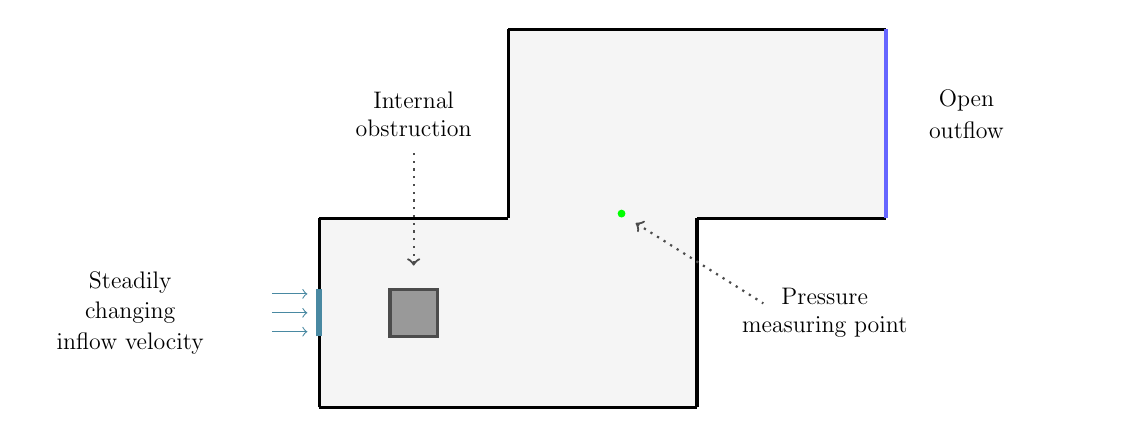
\begin{tikzpicture}
[
scale=0.6,
every node/.style ={scale=0.6},
Background/.style={rectangle,draw=black!04,fill=black!04, thin, minimum size = 4 cm},
Obstruction/.style={rectangle,draw=black!70,fill=black!40, very thick, minimum size=1cm},
Finegrid/.style={step=0.5cm,gray,very thin},
Thickline/.style={-,draw=black!100,fill=black!02, very thick},
Thinline/.style={draw=black!100,fill=black!02, very thin},
Inflow/.style={-,draw={rgb,255:red,73;green,137;blue,162},line width=0.8mm},
Inarrow/.style={->,draw={rgb,255:red,73;green,137;blue,162},thin},
Outflow/.style={-,draw=blue!60,very thick},
Ball/.style={circle, draw=black!40, fill=red!20, thin, minimum size=3.5mm},
Circle/.style={circle,draw=black!40,fill=black!06,thin,minimum size=35.5mm},
Rectangle/.style={rectangle,draw=black!10,fill=white,inner xsep=0pt, inner ysep=0pt,},
Box/.style = {very thin, rectangle, inner xsep=10pt, inner ysep=10pt,},
%Device/.style={fill={rgb,255:red,192;green,58;blue,10}, draw={rgb,255:red,192;green,58;blue,10}},
Device/.style={fill=green, draw=green},
Arrow/.style={thick, dotted, draw=black!70}
]

\node[Background] at (2,2) {};
\node[Background] at (6,2) {};
\node[Background] at (6,6) {};
\node[Background] at (10,6) {};

\node[Obstruction] at (2,2) {};

\draw[Thickline] (0,0)--(8,0);
\draw[Thickline] (4,8)--(12,8);
\draw[Thickline] (0,4)--(4,4);
\draw[Thickline] (8,4)--(12,4);

\draw[Thickline] (0,0)--(0,4);
\draw[Thickline] (4,8)--(12,8);
\draw[Thickline] (4,4)--(4,8);
\draw[Thickline] (8,0)--(8,4);
\draw[Thickline] (12,4)--(12,8);

\draw[Inflow]   (0,1.5)--(0,2.5);
\draw[Inarrow]  (-1,1.6)--(-0.25,1.6);
\draw[Inarrow]  (-1,2.0)--(-0.25,2.0);
\draw[Inarrow]  (-1,2.4)--(-0.25,2.4);
\draw[Outflow]  (12,4)--(12,8);

\draw[Device] (6.4,4.1) circle (2pt);
\draw [<-, Arrow] (6.7,3.9) -- (9.4,2.2);
\draw [<-, Arrow] (2.0,3.0) -- (2.0,5.4);
\node [Box] (Box) at (-4.0,2.0)  {\begin{minipage}{0.3\textwidth}\centering{\Large Steadily changing\\[0.8ex] inflow velocity}\end{minipage}};
\node [Box] (Box) at (13.7,6.2){\begin{minipage}{0.4\textwidth}\centering{\Large Open \\[0.8ex] outflow}\end{minipage}};
\node [Box] (Box) at (2.0,6.2)  {\begin{minipage}{0.4\textwidth}\centering{\Large Internal \\[0.8ex] obstruction}\end{minipage}};
\node [Box] (Box) at (10.7,2.0){\begin{minipage}{0.4\textwidth}\centering{\Large Pressure  \\[0.8ex] measuring point}\end{minipage}};
\end{tikzpicture}


%\includegraphics[width=0.5\textwidth]{pictures/pipe4_0155_single.png}
\end{center}
\caption[{\ct poisson2d} test case]{{\ct poisson2d} test case consisting of a 2D-pipe geometry with a small obstruction and steadily changing inflow conditions.}
\label{FIG_scarc_poisson_geometry}
\end{figure}

As already explained in detail in Section (\ref{SEC_SCARC_poisson}), parallel elliptic solvers usually have trouble to map global information transfer correctly. Just this effect shall be examined here in terms of accuracy and convergence speed. 
To this end, air is blown into the domain whereby the inflow velocity is continuously varied within a range of 0 to 2 $m/s$
such that the flow pattern in the entire domain frequently changes. As will be seen in the later plots this RAMP-based setting will cause a very characteristic course for the pressure trace which is measured in the green indicated device in the middle of the domain up to the final simulation time of 0.5~s.
%
The need to continuously adapt to varying global situations poses a particular challenge to the pressure solver and is intentionally used to analyze the related scalability of the different variants with respect to an increasing number of meshes.
To this end, two different variants for this case will be analyzed subsequently which differ in the number of used meshes and the underlying grid resolutions.

% -------------------------------------------------------------------------------------------------------------------------------
% Pressure_Solver/poisson2d_4mesh
% -------------------------------------------------------------------------------------------------------------------------------
\subsubsection{Subdivision into 4 meshes ({\ct poisson2d\_4mesh})}
\label{SEC_SCARC_poisson_four}

In this case the pipe geometry from Figure \ref{FIG_scarc_poisson_geometry} is subdivided into 4 meshes with a side length of 40~cm  each. The single meshes are refined into $16^2$ cells corresponding to a grid resolution of 2.5~cm. The resulting flow field at time $t=0.31$ is illustrated in Figure \ref{FIG_scarc_poisson_four_flowfield}.
%
For the grid resolution considered here, the structured \fftdefault{} and \scarcdefault{} are based on a 
default velocity tolerance 0.0125 $m/s$, while \ffttight{} and \scarctight{} apply the finer tolerance 0.00001 $m/s$.
No velocity tolerance is needed for both unstructured variants \uglmat{} and \uscarc{}. 


\begin{figure}[ht]
\begin{center}
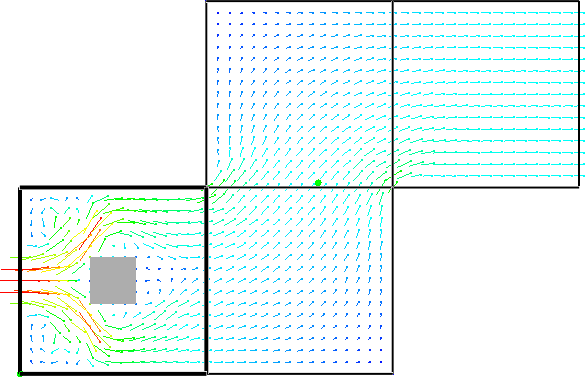
\includegraphics[width=0.5\textwidth]{\figPath/poisson2d_4mesh/poisson2d_4mesh_flowfield}
\end{center}
\caption[Flow field for a 4-mesh subdivision of the poisson2d test case]{Flow field for a 4-mesh subdivision of the poisson2d test case at $t=0.31$.}
\label{FIG_scarc_poisson_four_flowfield}
\end{figure}


The pressure traces which were measured for these six different solvers in the indicated device
are illustrated in Figure (\ref{FIG_SCARC_poisson_four_trace}).
Note, that the observed stair-like course correlates to the alternating strengths of the inflow velocity.
As a globally operating direct method, \uglmat{} provides an exact solution to the Poisson problem in each time step. Thus, its pressure trace is regarded as a reference solution for all other solvers.

\begin{figure}[ht]
\begin{center}
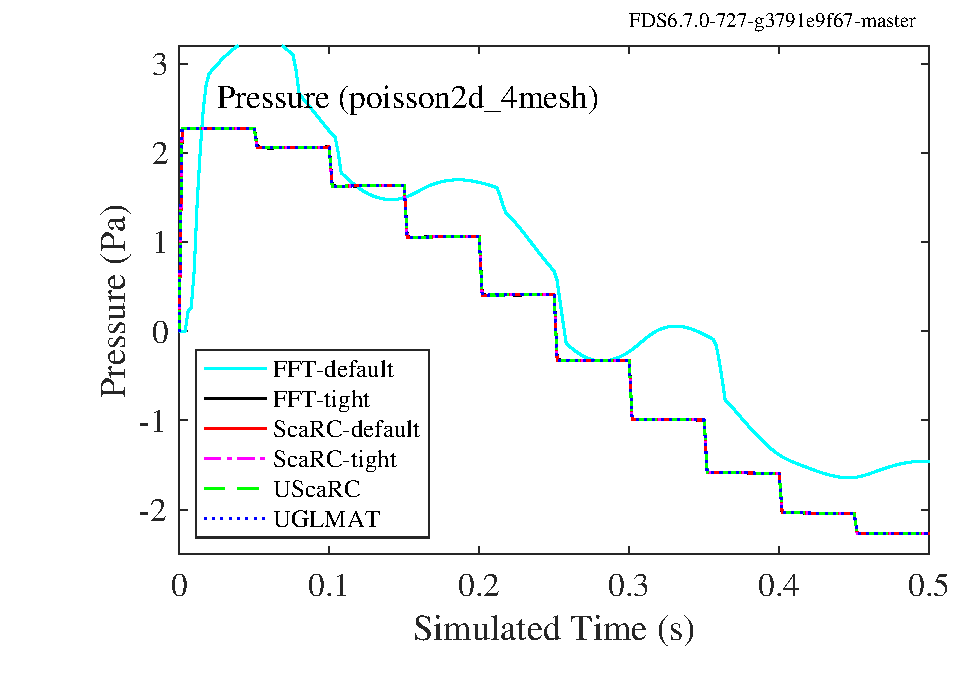
\includegraphics[width=3in]{\figPath/poisson2d_4mesh/poisson2d_4mesh_pres}
\end{center}
\caption[Pressure traces of the different pressure solvers for {\ct poisson2d} with 4 meshes]{Pressure traces of the different pressure solvers for {\ct poisson2d} with 4 meshes. }
\label{FIG_SCARC_poisson_four_trace}
\end{figure}

Obviously \fftdefault{} (cyan) has troubles to map the pressure trace correctly while \scarcdefault{} (red) 
already seems to match exactly. Both are structured solvers which are not able to set the correct boundary values along the inner obstruction by design. However, this basically doesn't seem to carry much weight here, as can be seen for \scarcdefault{} for which the obstruction is the only possible error influence in this test case.
With a view to the constantly changing global velocity field, the multi-mesh decomposition seems to cause much more troubles 
which is reflected in the serpentine line of \fftdefault{}. The steady changes of the inflow conditions can only be spread across the entire domain by successive mesh-by-mesh communications. Thus, the new inflow information reaches the pressure device in the third mesh only with delay. Evidently, this cannot be sufficiently remedied by the default pressure iteration.

However, as observed for \ffttight{} (black), the tighter pressure iteration works great and is able to completely resolve these troubles leading to a correct pressure trace if only a higher number of pressure iterations is performed.
In contrast to this, there seems to be no reason at all to apply \scarctight{} in this case. Since all \scarc{} variants provide correct transitions at mesh interfaces by design, the overall error influences are significantly less pronounced here.
Finally, \uscarc{} (green dashed) operates independently of all these effects and produces the same correct pressure trace as \uglmat{} (blue dotted).

So far, Figure (\ref{FIG_SCARC_poisson_four_trace}) reflects the accuracy which is achieved by the different solvers in the approximation of the pressure trace, but it does not say anything about the numerical effort required for this.
While for both unstructured solvers \uglmat{} and \uscarc{} only one pressure iteration is needed by construction, the structured variants require the execution of different numbers of pressure iterations until the respective velocity tolerance is met. 
In order to analyze this situation in more detail,  
the achieved accuracies for the velocity errors, as displayed in Figure \ref{FIG_SCARC_poisson_four_velerror}, are set in relation to
the number of pressure iterations required to reach them, as displayed in Figure \ref{FIG_SCARC_poisson_four_presite}.

\begin{figure}[ht]
\begin{center}
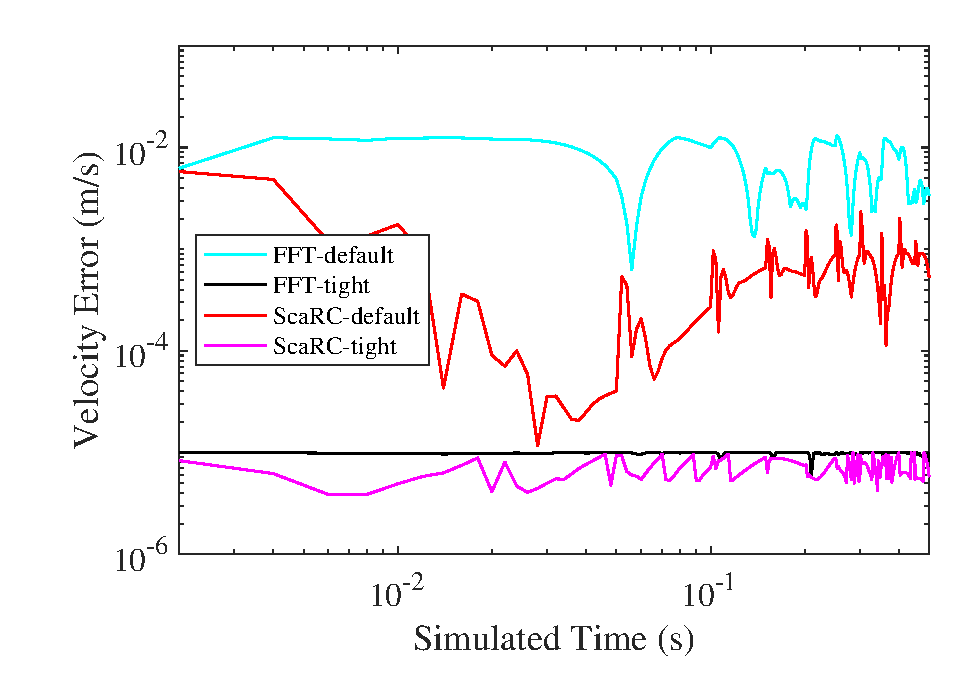
\includegraphics[width=3in]{\figPath/poisson2d_4mesh/poisson2d_4mesh_velerror}\\
\end{center}
\caption[Velocity tolerances of the structured pressure solvers in case of the 4-mesh poisson2d test case]{Velocity tolerances of the structured pressure solvers for {\ct poisson2d} with 4 meshes.}
\label{FIG_SCARC_poisson_four_velerror}
\end{figure}

\begin{figure}[ht]
\begin{center}
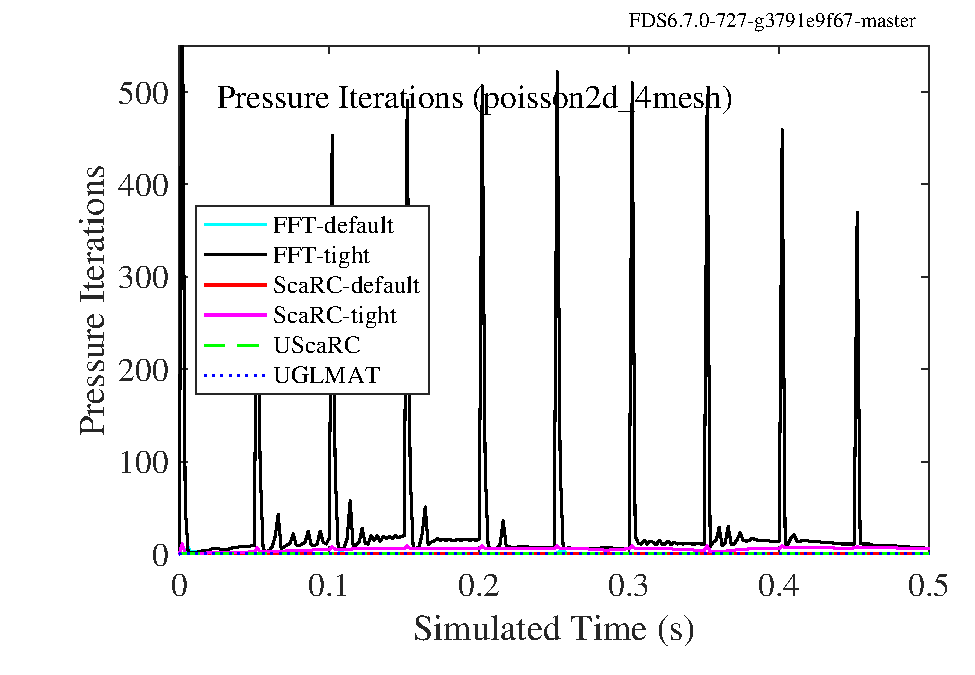
\includegraphics[width=3in]{\figPath/poisson2d_4mesh/poisson2d_4mesh_presite}
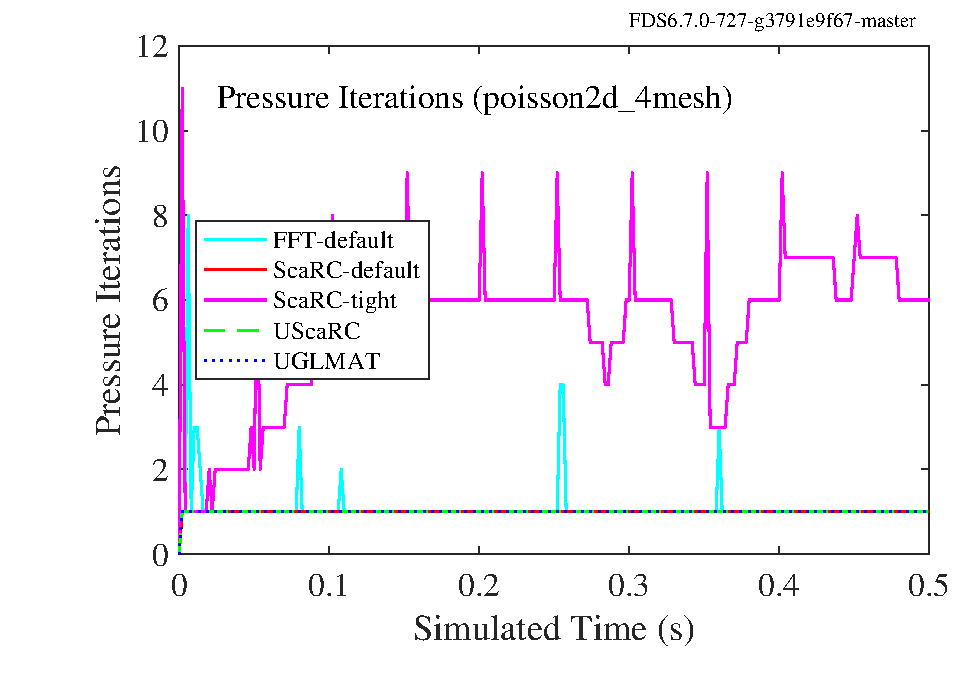
\includegraphics[width=3in]{\figPath/poisson2d_4mesh/poisson2d_4mesh_presite_zoom}
\end{center}
\caption[Pressure iterations of the different pressure solvers for {\ct poisson2d} with 4 meshes]{Pressure iterations of the different pressure solvers for {\ct poisson2d} with 4 meshes.  (Left) Comparison of all solvers. (Right) Zoomed view  without \ffttight{}.}
\label{FIG_SCARC_poisson_four_presite}
\end{figure}

Note, that Figure \ref{FIG_SCARC_poisson_four_velerror} only illustrates the velocity tolerances for the structured solvers because \uglmat{} and \uscarc{} achieve machine precision in the range of $10^{-16}$ by design which is omitted here to allow a more diversified view of the remaining solvers. Similarly, while the left plot in Figure \ref{FIG_SCARC_poisson_four_presite} compares the pressure iterations for all six solvers, the right plot omits \ffttight{} in order to give a more detailed overview of the others.

According to the size of the default velocity tolerance, \fftdefault{} (cyan) leads to a coarse velocity error in the range of about $10^{-2}$ as can be seen in Figure \ref{FIG_SCARC_poisson_four_velerror}.  
This error consists of two parts, namely the accuracy along the internal obstruction and the accuracy at the mesh interfaces. The related pressure iteration mostly converges within 1 cycle. Only with changing inflow conditions occasionally up to 4 cycles are needed as can be seen at the cyan line in the right plot of Figure \ref{FIG_SCARC_poisson_four_presite}. The maximum number of 8 cycles is only required at the beginning of the simulation until the flow field has built up for the first time, but never again after. Thus, convergence is fast, but it is also associated with the error of the pressure trace displayed in Figure \ref{FIG_SCARC_poisson_four_trace}.

Although its surrounding pressure iteration is based on the same default velocity tolerance, 
\scarcdefault{} (red) already provides a basically smaller velocity error compared to \fftdefault{} in the range of about $10^{-4}$ up to $10^{-3}$, see Figure \ref{FIG_SCARC_poisson_four_velerror} again.
This is because the only part that makes up this error relates to the inner obstruction, whereas nothing is added at mesh interfaces any more.  Convergence can always be achieved in just 1 pressure iteration independently of the inflow changes and there is no major fluctuation at the beginning. 

Figure \ref{FIG_SCARC_poisson_four_velerror} also proves that
\ffttight{} (black) and \scarctight{} (magenta) succeed to fulfill the required velocity tolerance of $10^{-5}$. 
However, when looking to Figure \ref{FIG_SCARC_poisson_four_presite} the biggest difference between both solvers becomes apparent: While \ffttight{} needs relatively many pressure iterations (averagely 35) to fulfill the fine tolerance, \scarctight{} requires considerably less (averagely 6). 
Note, that the average calculation was restricted to the time interval $[0.05,0.5]$ such that the higher fluctuations which only occur
at the beginning were neglected in order not to falsify the whole picture.
In particular, at every change of the inflow conditions, the latency of \ffttight{} gets obvious in a short-term increase of the number of iterations (up to 522 in the worst case) which basically relies on the fragmentation induced by the subdivision. 

In fact, the right plot in Figure \ref{FIG_SCARC_poisson_four_presite} also reveals slight increases of \scarctight{} for every inflow change, because it still has to prevent the velocity penetration into the internal obstruction. However this is significantly less than for \ffttight{} and a maximum of 11 iterations is never exceeded.
This difference again reflects the fact that the subdivision is already captured correctly by \scarc{} and that the only disturbing influences are caused by the internal obstruction.
%
As expected, \uglmat{} (blue dotted) and \uscarc{} (green dashed)
produce machine precision accuracy and both need exactly one pressure iteration.



% -------------------------------------------------------------------------------------------------------------------------------
% Pressure_Solver/poisson2d_16mesh
% -------------------------------------------------------------------------------------------------------------------------------
\subsubsection{Subdivision into 16 meshes ({\ct poisson2d\_16mesh})}
\label{SEC_SCARC_poisson_sixteen}

To analyze the scalability towards higher mesh numbers the pipe geometry of Figure \ref{FIG_scarc_poisson_geometry} is now subdivided into 16 meshes with a side length of 20~cm  each. Furthermore, a finer grid resolution for the single meshes into $32^2$ cells is used which corresponds to a grid resolution of 0.625~cm. The respective default velocity tolerance for the structured solvers FFT and \scarc{} amounts to 0.3125~cm, while the fine velocity tolerance of 0.00001 $m/s$ is used again.
The resulting flow field at time $t=0.31$ is illustrated in Figure \ref{FIG_scarc_poisson_four_flowfield}.


\begin{figure}[ht]
\begin{center}
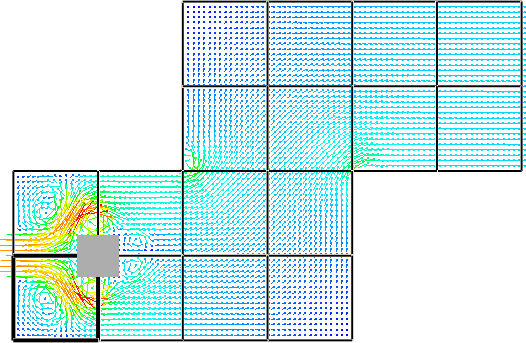
\includegraphics[width=0.5\textwidth]{\figPath/poisson2d_16mesh/poisson2d_16mesh_flowfield}
\end{center}
\caption[Flow field for {\ct poisson2d} with 16 meshes]{Flow field for {\ct poisson2d} with 16 meshes at $t=0.31$.}
\label{FIG_scarc_poisson_sixteen_flowfield}
\end{figure}

Subsequently, similar plots for the pressure traces, velocity errors and required number of pressure iterations will be presented as already done for the 4-mesh subdivision before. 
To this end, the left plot in Figure \ref{FIG_SCARC_poisson_sixteen_trace} shows the measured pressure traces over the whole simulation time $[0,0.5]$. Obviously, the already known stair-like course of the pressure trace is still overlaid with small oscillations which are captured differently well by the various pressure solvers. To better illustrate their resolution qualities, the right plot of Figure \ref{FIG_SCARC_poisson_sixteen_trace} also gives a zoomed view to the time interval $[0.29, 0.302]$.

\begin{figure}[ht]
\begin{center}
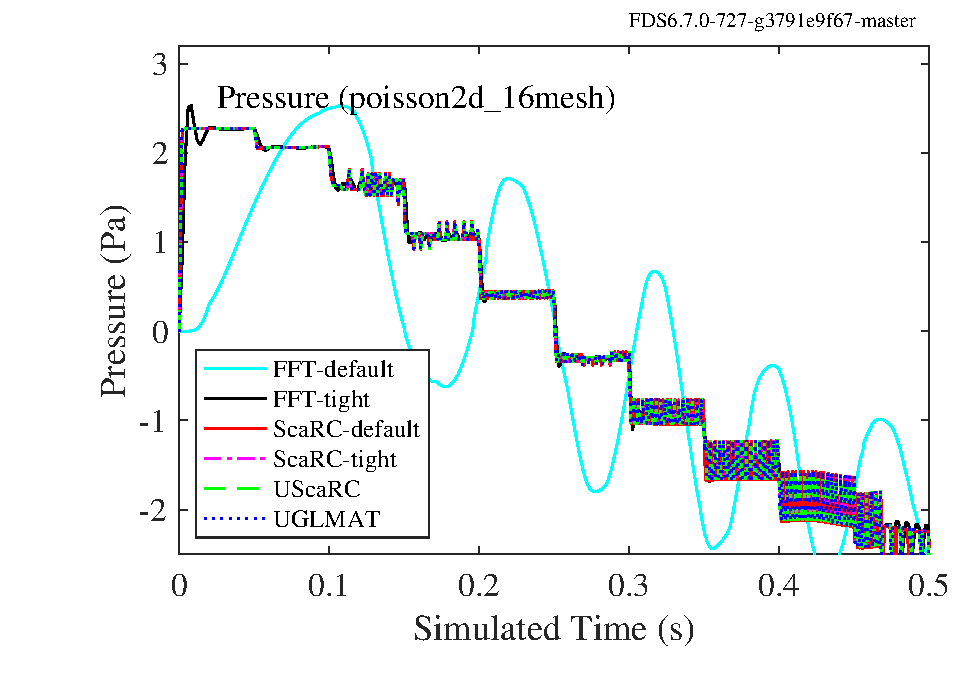
\includegraphics[width=3in]{\figPath/poisson2d_16mesh/poisson2d_16mesh_pres}
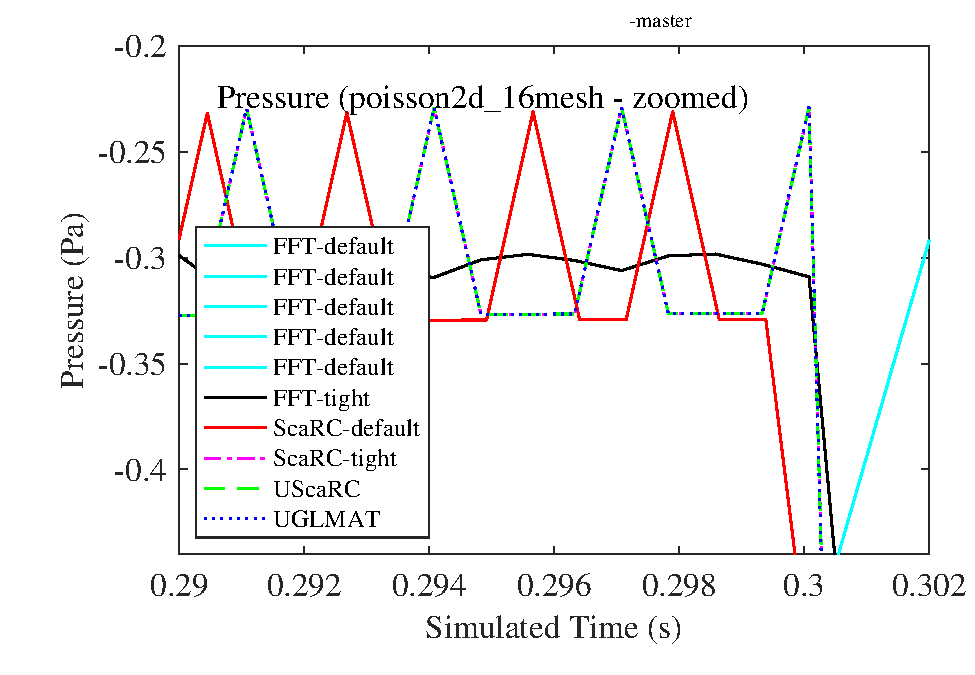
\includegraphics[width=3in]{\figPath/poisson2d_16mesh/poisson2d_16mesh_pres_zoom}
\end{center}
\caption[Pressure traces of the different pressure solvers for {\ct poisson2d} with 16 meshes]{Pressure traces of the different pressure solvers for {\ct poisson2d} with 16 meshes. (Left) Whole time interval $[0.0, 0.5]$. (Right) Zoomed view to time interval $[0.29, 0.302]$.}
\label{FIG_SCARC_poisson_sixteen_trace}
\end{figure}

As expected, the higher number of meshes poses an even greater challenge for \fftdefault{} (cyan) to correctly map the pressure trace as can be seen in the left plot of Figure \ref{FIG_SCARC_poisson_sixteen_trace}. Thus, the use of a tighter velocity tolerance for the FFT solver seems to be indispensible. In fact, the zoomed view on the right reveals that \ffttight{} (black) is close to the correct pressure course as indicated by \uglmat{}, but still doesn't completely match the small oscillations. However, to reach this approximate consistency, it already requires a large number of pressure iterations, see the left plot of Figure \ref{FIG_SCARC_poisson_sixteen_presite}. 
While  on average 642 pressure iterations have to be performed, the maximum available number of 1000 pressure iterations is often not sufficient to map the fine velocity criterion of $10^{-5}$ and occasionally only a lower accuracy can be achieved. This is also illustrated in Figure \ref{FIG_SCARC_poisson_sixteen_velerror} which displays the achieved velocity errors for all structured solvers. Obviously, the black  \ffttight{} line has a hard time falling below the $10^{-5}$ line.
When comparing the different plots therein, please note that the velocity errors for both \scarc{} variants only result from the penetration error towards the internal obstruction while the velocity errors for the FFT variants are a combination of both the error at the internal obstruction and at mesh interfaces.


\begin{figure}[ht]
\begin{center}
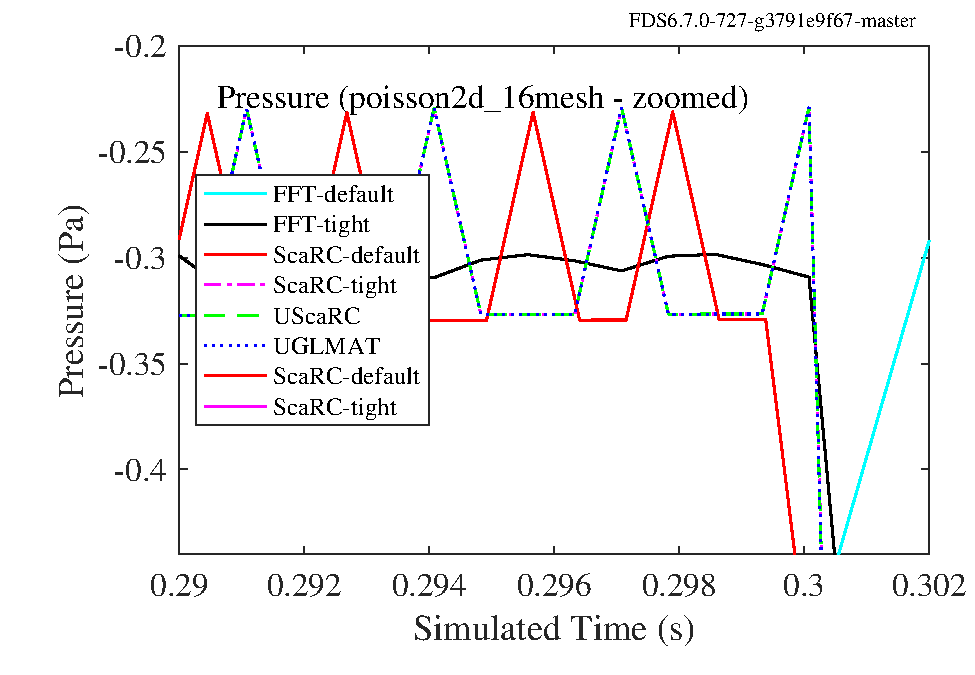
\includegraphics[width=3in]{\figPath/poisson2d_16mesh/poisson2d_16mesh_velerror}\\
\end{center}
\caption[Achieved velocity tolerances for the structured solvers in case of the 16-mesh poisson2d test case]{Achieved velocity tolerances for the structured solvers for {\ct poisson2d} with 16 meshes.}
\label{FIG_SCARC_poisson_sixteen_velerror}
\end{figure}

\begin{figure}[ht]
\begin{center}
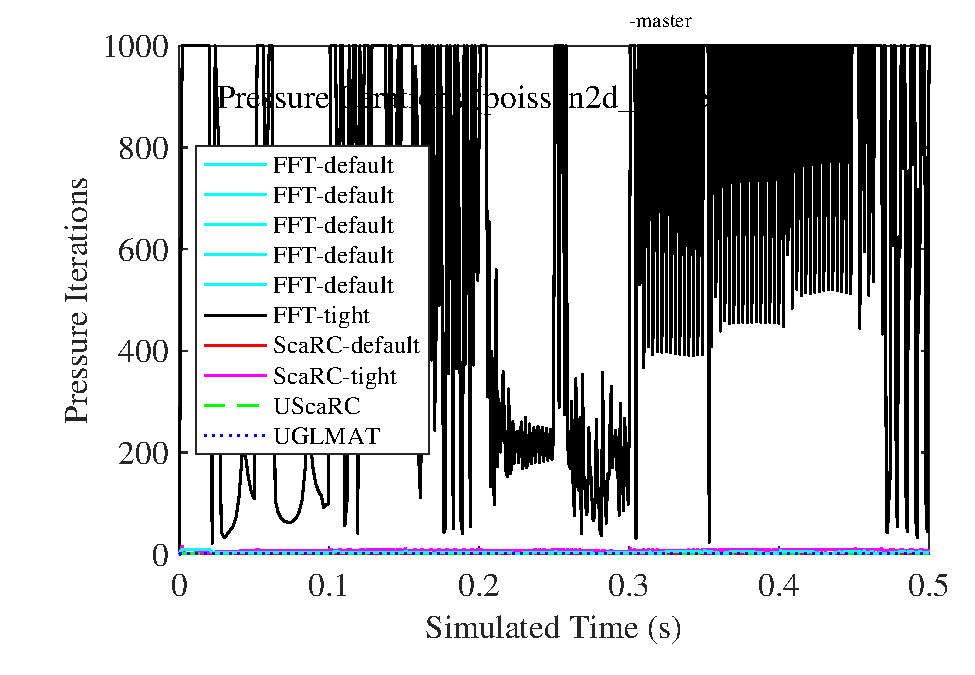
\includegraphics[width=3in]{\figPath/poisson2d_16mesh/poisson2d_16mesh_presite}
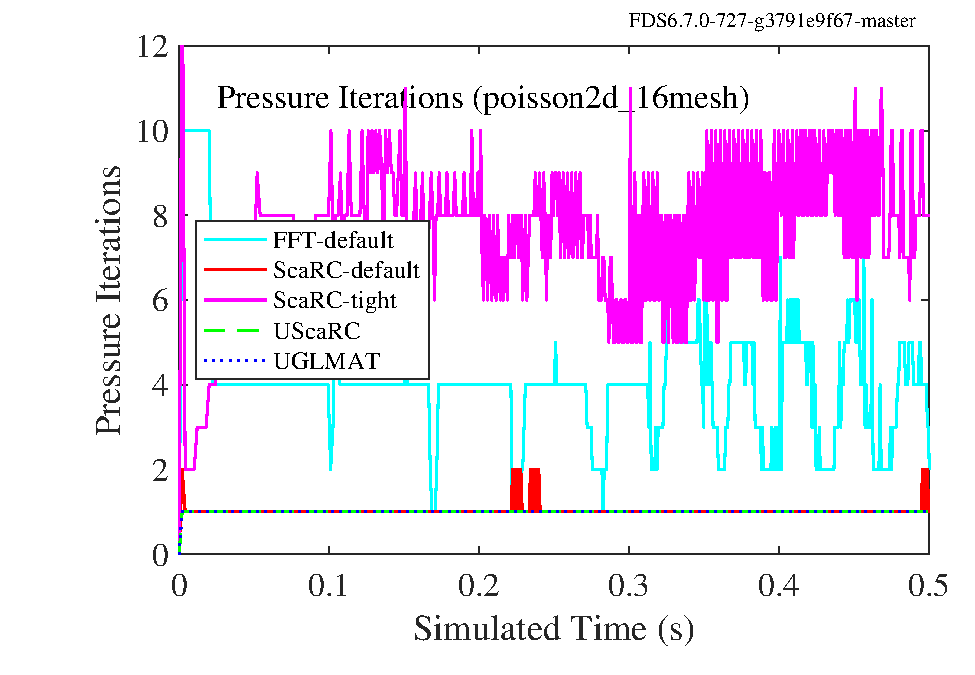
\includegraphics[width=3in]{\figPath/poisson2d_16mesh/poisson2d_16mesh_presite_zoom}
\end{center}
\caption[Number of required pressure iterations of the different pressure solvers for {\ct poisson2d} with 16 meshes]{Number of required pressure iterations of the different pressure solvers for {\ct poisson2d} with 16 meshes. (Left) Comparison of all six solvers. (Right) Zoomed view  without \ffttight{}.}
\label{FIG_SCARC_poisson_sixteen_presite}
\end{figure}

Furthermore, the right plot in Figure \ref{FIG_SCARC_poisson_sixteen_trace} proves that \uscarc{} (green dashed) and \scarctight{} (magenta) produce the same exact pressure trace as the reference solver \uglmat{}. While \uglmat{} and \uscarc{} just require 1 pressure iteration by design, \scarctight{} needs only 7 pressure iterations on average and 11 in maximum to fulfil the tight velocity tolerance, see the related number of pressure iterations in the right plot of Figure \ref{FIG_SCARC_poisson_sixteen_presite} and the  velocity tolerance  in Figure \ref{FIG_SCARC_poisson_sixteen_velerror} which is completely below $10^{-5}$.
%
Since \scarctight{} already provides correct inter-mesh transitions by design, it not only requires significantly less pressure iterations than \ffttight{}, but it also reliably achieves the desired velocity tolerance.
Even \scarcdefault{} (red) seems to be in the correct order of magnitude and only needs 1 pressure iteration in average (and only very rarely 2), however its pressure trace still shows the slight offset to the correct course indicating that the default tolerance isn't just fully sufficient to handle the internal obstruction.

In conclusion, in this case the domain decomposition seems to be far more difficult to handle than the internal obstruction.
However, these observations do not represent a general rule. That the situation can be completely different and that the inner obstructions may have a greater influence than the mesh decomposition becomes apparent subsequently in the {\ct {\ct duct\_flow}} case.


% ---------------------------------------------------------------------------------
% Generalized \scarc{} solvers for the poisson2d case
% ---------------------------------------------------------------------------------
\subsubsection{Application of generalized \scarc{} solvers}
\label{SEC_SCARC_poisson_generalizations}

As explained in detail in Section (\ref{SEC_SCARC_generalizations}) there are multiple possibilities to generalize the \scarc{} solver. 
The different \scarc{} variants, which were used for the multi-mesh {\ct poisson2d} computations so far, were all 
based on a global data-parallel CG-method with different types of preconditioning. 
Two further variants, \scarctwolevel{} and \scarcmultigrid{}, were introduced at the beginning of Section (\ref{SEC_SCARC_verification})
which are now also applied to the {\ct poisson2d} case in order to give an impression of their properties and performance. 
Both are based on structured discretizations. While also using a global CG-method, \scarctwolevel{} relies on a \tls{}-preconditioner whose additional coarse grid is based on one refinement of the domain decomposition itself. \scarcmultigrid{} uses a global MG-method instead with smoothing by local SSOR-methods, again with a coarse grid based on one refinement of the domain decomposition and additionally all intermediate grid levels in-between.

Since it was shown above that \uscarc{} gives the same correct result as \uglmat{}, the presentations in this subsection will only refer to different \scarc{} versions where \uscarc{} is used as reference. For the 16-mesh decomposition of {\ct poisson2d}, again with the fine grid resolution of 0.625~cm, Figure (\ref{FIG_scarc_poisson_sixteen_scarc_variants_trace}) compares the pressure traces for the unstructured \uscarc{} (green) with the structured \scarcdefault{} (red dashed), \scarctwolevel{} (cyan dash-dotted), \scarcmultigrid{} (blue dotted) where the later two were applied for the default velocity tolerance, too.

\begin{figure}[ht]
\begin{center}
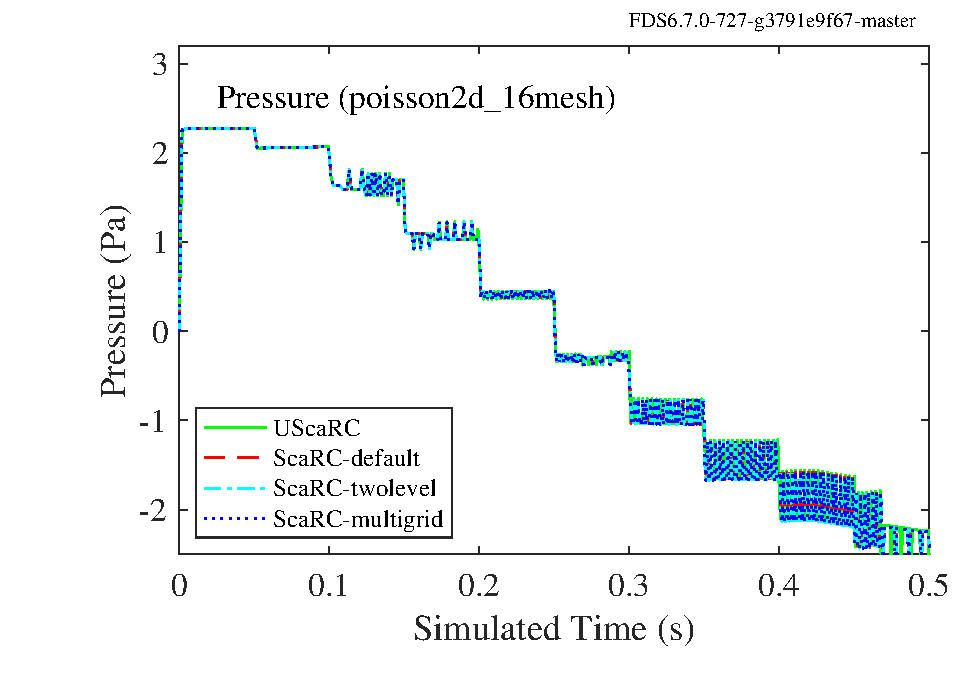
\includegraphics[width=3in]{\figPath/poisson2d_16mesh/poisson2d_16mesh_scarc_pres}
\end{center}
\caption[Pressure traces of different \scarc{} variants for {\ct poisson2d} with 16 meshes]{Pressure traces of different \scarc{} variants for {\ct poisson2d} with 16 meshes.}
\label{FIG_scarc_poisson_sixteen_scarc_variants_trace}
\end{figure}

A zoomed view to the interval $[0.29,0.302]$ is also given in the left plot of Figure (\ref{FIG_scarc_poisson_sixteen_scarc_variants_zoom}). Obviously, all default structured \scarc{} variants identically produce the same pressure trace which proves their basic correctness. But all show a slight offset compared to the correct pressure trace given by \uscarc{}, which has already been observed in Figure \ref{FIG_SCARC_poisson_sixteen_trace}. Again, this is based on their structured nature and the associated inaccuracy along the internal obstruction which obviously cannot be completely eliminated by the default pressure iteration. However, using the tight pressure iteration instead, the shift disappears for all structured variants as can be seen in the right plot of Figure (\ref{FIG_scarc_poisson_sixteen_scarc_variants_zoom}). For all of them, this requires the same number of averagely 7 pressure iterations.

\begin{figure}[ht]
\begin{center}
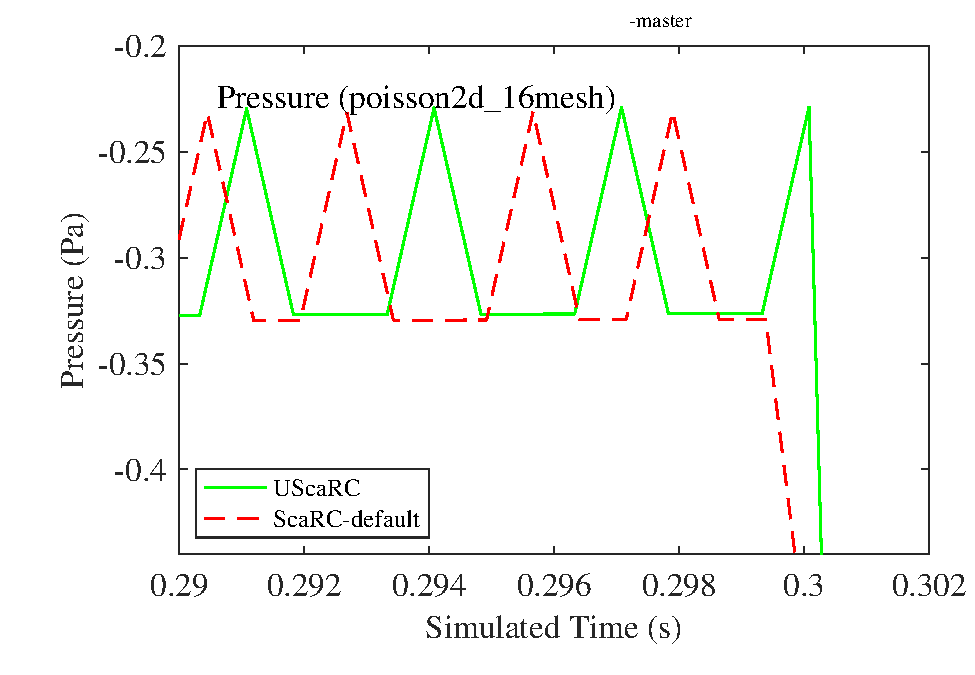
\includegraphics[width=3in]{\figPath/poisson2d_16mesh/poisson2d_16mesh_scarc_pres_zoom}
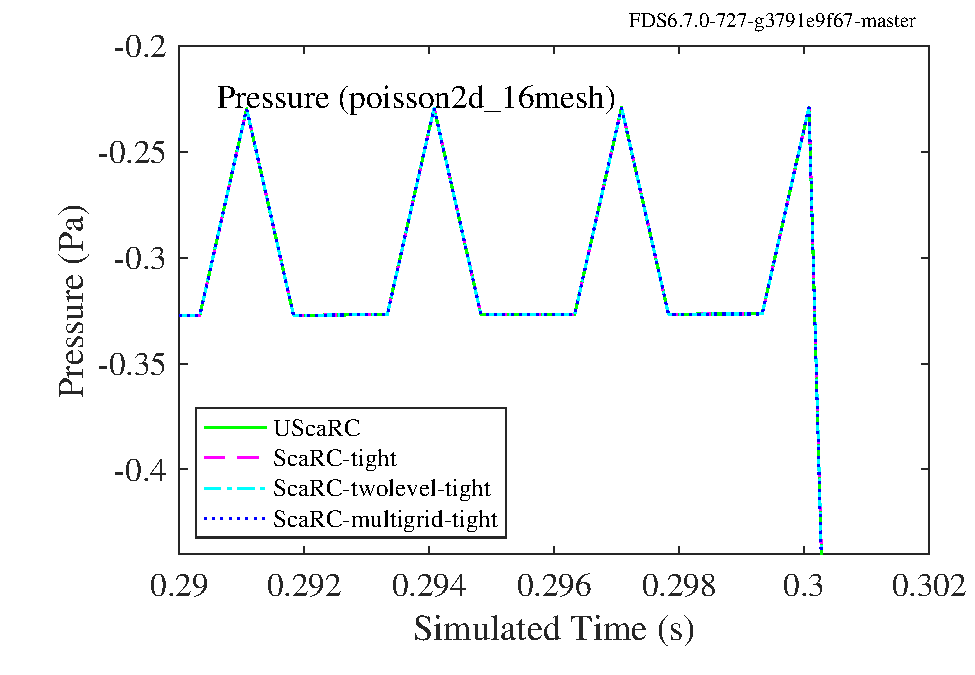
\includegraphics[width=3in]{\figPath/poisson2d_16mesh/poisson2d_16mesh_scarc_pres_tight_zoom}
\end{center}
\caption[Pressure traces of different \scarc{} variants for {\ct poisson2d} with 16 meshes]{Zoomed view of time interval $[0.29, 0.302]$ for the pressure traces of different \scarc{} variants for {\ct poisson2d} with 16 meshes. (Left) Default velocity tolerance. (Right) Tight velocity tolerance.}
\label{FIG_scarc_poisson_sixteen_scarc_variants_zoom}
\end{figure}


The focus of the subsequent investigations lies in the comparison of the achieved numerical efficiencies. 
The left plot in Figure (\ref{FIG_scarc_pi_twoD_scarc_convergence}) reveals that the convergence rates for the single \scarc{} variants
are quite different. The pure CG-variants, \uscarc{} and \scarcdefault{}, only achieve relatively bad convergence rates at 0.81, needing about 150 \scarc{} iterations per Poisson solution which is quite a lot and still needs further optimization.
Please note that if only a 4-mesh decomposition instead of the 16-mesh decomposition is used for the {\ct poisson2d} geometry while maintaining the same fine-grid resolution of 0.625~cm, a convergence rate of 0.7 at about 90 \scarc{} iterations is achieved,
which is still not good, but significantly better than for the 16-mesh case.

This observation reflects the fundamental design property of the \ols{} variants that their convergence quality decreases with increasing number of sub-meshes. An improvement can only be achieved by adding global information mechanisms as can be clearly observed with the \scarctwolevel{} variant (cyan). Here, the additional usage of a coarse grid level leads to a halving of the convergence rate to about 0.42, see the left plot of Figure (\ref{FIG_scarc_pi_twoD_scarc_convergence}). The right plot therein shows that this reduction is also associated with a comprehensive  reduction of the number of \scarc{} iterations from about 150 to 40, which is quite much because it has to be performed twice per FDS time step.  
Certainly, the single iterations are more expensive due to the additional computations and communications associated with the coarse grid problem what has to be kept in mind when comparing the different approaches.

\begin{figure}[ht]
\begin{center}
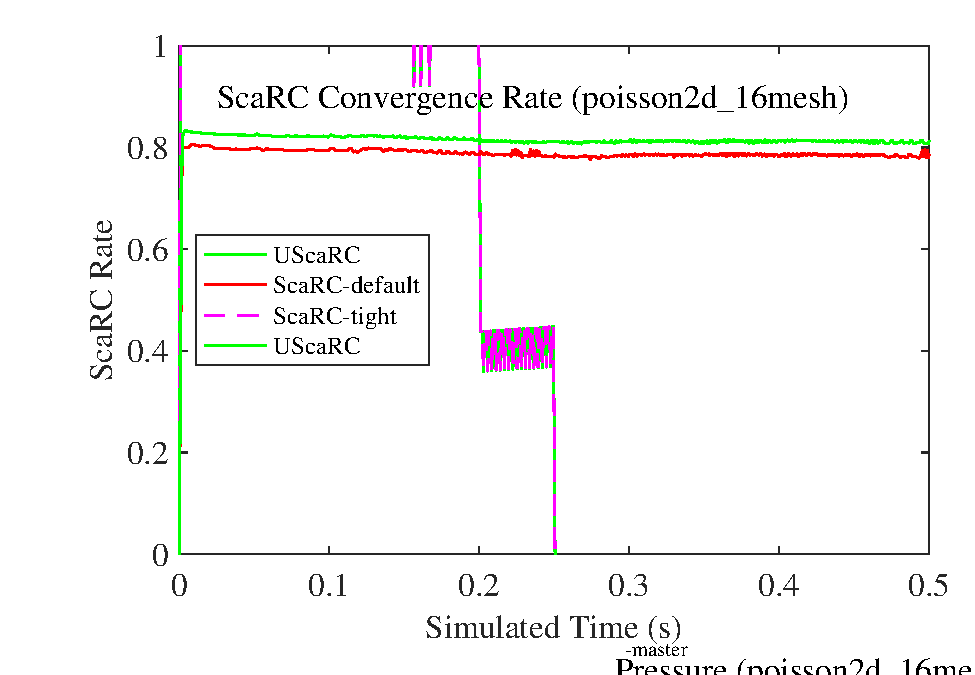
\includegraphics[width=3in]{\figPath/poisson2d_16mesh/poisson2d_16mesh_scarc_rate}
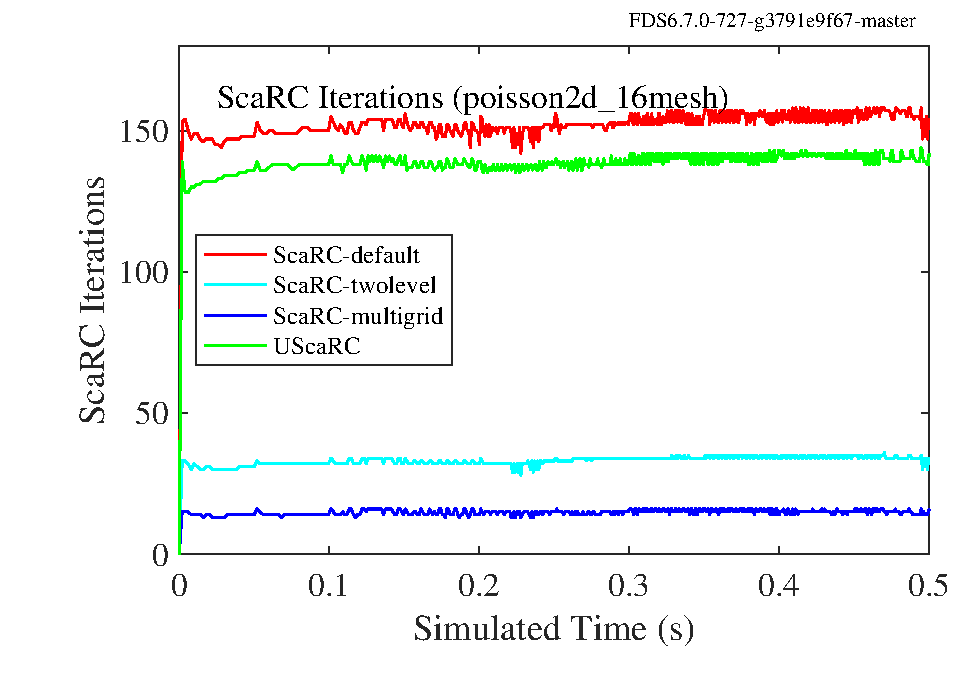
\includegraphics[width=3in]{\figPath/poisson2d_16mesh/poisson2d_16mesh_scarc_iter}
\end{center}
\caption[Comparison of the different \scarc{} variants] {Comparison of different \scarc{} variants for the 16-mesh {\ct poisson2d} case. (Left) \scarc{} convergence rates.  (Right) Number of required \scarc{} iterations. }
\label{FIG_scarc_pi_twoD_scarc_convergence}
\end{figure}


As expected the multigrid version shows by far the the smallest convergence rate in the range of 0.15 and requiring only about 15 \scarc{} iterations per Poisson solution. 
Here, the additional use of a coarse grid level and all intermediate levels in-between has a very positive effect on the global coupling. In practice, this typically leads to convergence rates which are more or less independent of the local grid refinement level and the number of sub-meshes.

There are numerous possibilities to vary the input parameters for the different \scarc{} variants, 
which may have a significant influence to the convergence speed. This especially holds true for \scarcmultigrid{}. 
So far, its smoothing consisted of only 2 SSOR-steps per grid level. 
It has already been explained in Section (\ref{SEC_SCARC_discussion}) that the accuracy achieved in solving the local problems has a major impact on the quality and convergence speed of the global solution. Hence, if the number of smoothing steps is increased, the finally required global number of \scarc{} iterations can further be decreased. Figure \ref{FIG_scarc_poisson_sixteen_multigrid} compares the resulting convergence rates and needed number of \scarc{} iterations for the use of 2, 3, 4 and 5 smoothing steps.

\begin{figure}[ht]
\begin{center}
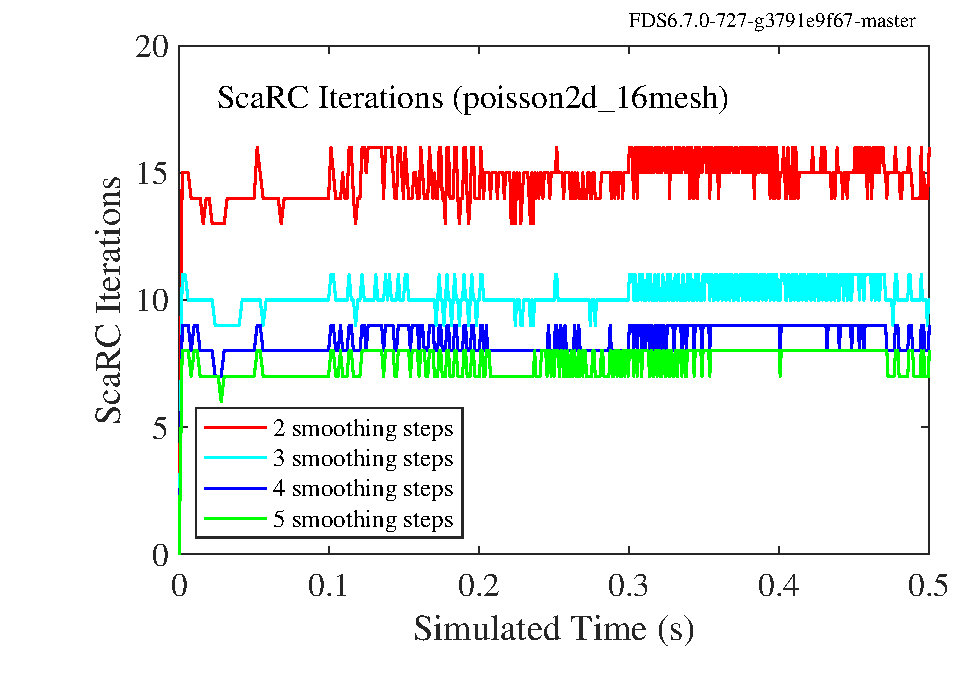
\includegraphics[width=3in]{\figPath/poisson2d_16mesh/poisson2d_16mesh_scarc_iter_gmg}
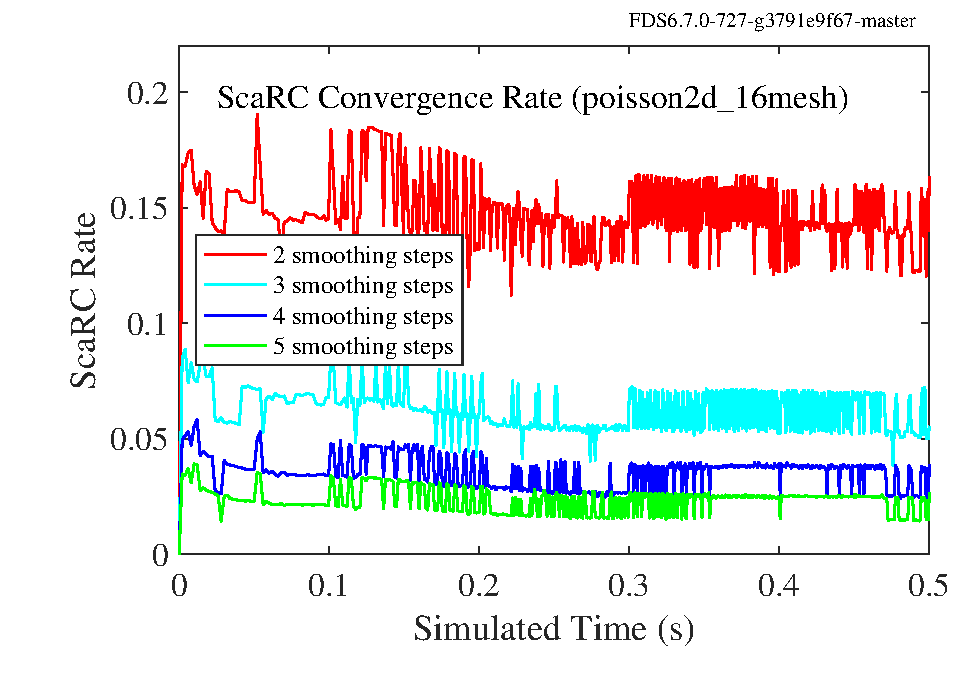
\includegraphics[width=3in]{\figPath/poisson2d_16mesh/poisson2d_16mesh_scarc_rate_gmg}
\end{center}
\caption[Convergence of \scarcmultigrid{} for different numbers of smoothing steps for {\ct poisson2d} with 16 meshes]{Convergence of \scarcmultigrid{} for different numbers of smoothing steps 
for {\ct poisson2d} with 16 meshes.
(Left) Required number of \scarc{} iterations. (Right) \scarc{} convergence rates.}
\label{FIG_scarc_poisson_sixteen_multigrid}
\end{figure}

Apparently, each additional smoothing step leads to a clear reduction of the achieved convergence rate and the number of required \scarc{} iterations. This amounts from 15 \scarc{} iterations with a convergence rate of 0.15 in case of 2 smoothing steps up to only 7 \scarc{}  iterations with a convergence rate of only 0.025 in case of 5 smoothing steps.
Note, that during the smoothing global matrix-vector products (including local communication) are needed. Thus, the use of additional smoothing cycles leads to a corresponding increase of work. But at the same time, the number of coarse grid solutions (including global communication) is comprehensively reduced 
which in turn represents a major saving and usually makes up for the extra cost.

\subsubsection{Preliminary conclusions}
\label{SEC_SCARC_poisson_evaluation}
The cases just presented have shown that there is a wide range of \scarc{} variants that can be used to solve the Poisson equation. These differ significantly in the type of the underlying discretization, the preconditioning mechanisms used, and whether they work only at the fine grid level or at additional coarser grid levels. The biggest difference to the current FFT solver consists in the fact that \scarc{} has no more errors along inner mesh boundaries. Thus, for the structured \scarc{} variants often much less pressure iterations are needed than for the default FFT solver, because it only has to take care of the reduction of the penetration error towards inner obstructions. For the unstructured variant \uscarc{}, no pressure iteration at all is needed anymore.

As a basis for all further developments, the focus of the previous analyses has been on proving the fundamental correctness of the various \scarc{} approaches. For this purpose the case {\ct poisson2d} was developed and tested in the above as well as many other ways. Corresponding 3D studies related to geometries with one or more internal obstructions and with subdivisions into different numbers of meshes were also carried out. However, since it was not possible to gain any insights beyond those shown so far, no presentation of these cases has currently been made. Instead, the coming test series will concentrate on the official FDS verification and validation cases to examine the suitability of \scarc{} for more realistic cases.

The previous studies have shown that the addition of coarser grid levels can contribute to a significant improvement of numerical efficiency. However, the achieved convergence acceleration must be put in relation to the increased costs for each single iteration.
A final assessment for the performance of the different variants can only be done on the base of additional measurements of the computational times. 
In order to arrive at meaningful estimates for the optimal parameters a-priori, different sensitivity studies are in work which should finally allow to identify an optimal set of parameters that delivers resilient and efficient results for a large number of general cases.
Some of the most recent tests, which have already been carried out for various validation cases, suggest that
there is still a need for further optimisation with regard to the required running times which is currently in progress.

\newpage
% ======================================================================================
% dancing_eddies case
% ======================================================================================
\subsection{Karman vortex street}
\label{SEC_SCARC_dancing_eddies}

\subsubsection{Subdivision into 4 meshes ({\ct dancing\_eddies})}
The following computations refer to the {\ct dancing\_eddies} case from the Pressure\_Solver verification directory. It concerns a 30~cm long, two-dimensional channel with a grid resolution of 0.1~cm which is subdivided into 4 meshes. Air is pushed into the channel at 0.5~m/s. A flat obstruction in the left third of the channel causes the formation of a Karman vortex street. Figure \ref{FIG_scarc_dancing_eddies_four} displays a contour plot of the pressure at the final simulation time t=2~s.
\begin{figure}[ht]
\begin{center}
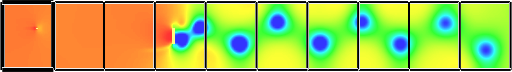
\includegraphics[width=0.9\textwidth]{\figPath/dancing_eddies/dancing_eddies_geometry}
\end{center}
\caption[Contour plot for the 4-mesh {\ct {\ct dancing\_eddies}} case]{Contour plot of the pressure for \uscarc{} after 2~s in case of a 4-mesh subdivision.}
\label{FIG_scarc_dancing_eddies_four}
\end{figure}

The original test case compares the structured solvers \fftdefault{} (with the default velocity tolerance of 0.0005~m/s) and \ffttight{} (with the finer tolerance of 0.00001~m/s) with the unstructured direct solver \uglmat{}. These tests are now extended by the application of the structured solvers \scarcdefault{} and \scarctight{} (both with the same velocity tolerance settings as their FFT counterparts) as well as the unstructured \uscarc{}. 
As in the original case, the computed pressure traces are compared with the corresponding single mesh solution which is used as reference solution here, see Figure \ref{FIG_scarc_dancing_eddies_pressure}.

\begin{figure}[ht]
\begin{center}
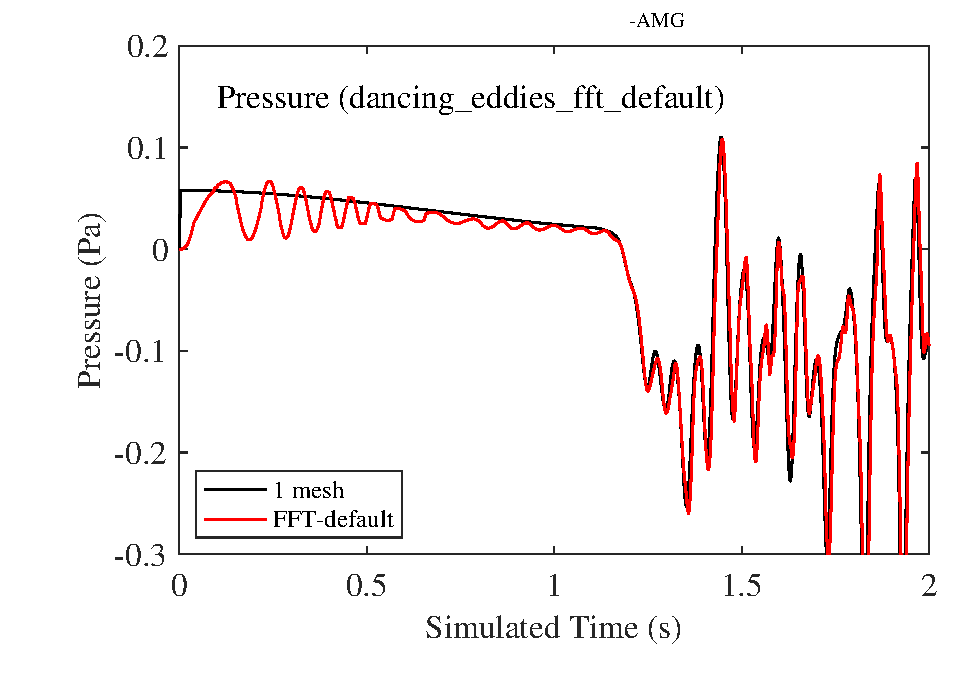
\includegraphics[width=3in]{\figPath/dancing_eddies/dancing_eddies_default}
\includegraphics[width=3in]{\figPath/dancing_eddies/dancing_eddies_scarc}
%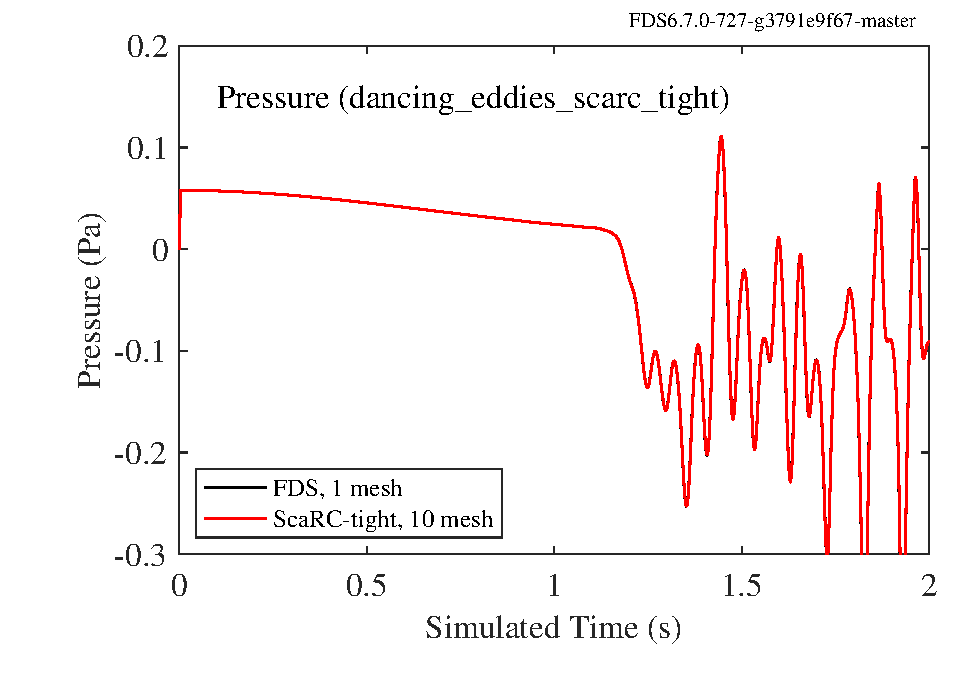
\includegraphics[width=3in]{\figPath/dancing_eddies_scarc_tight}
%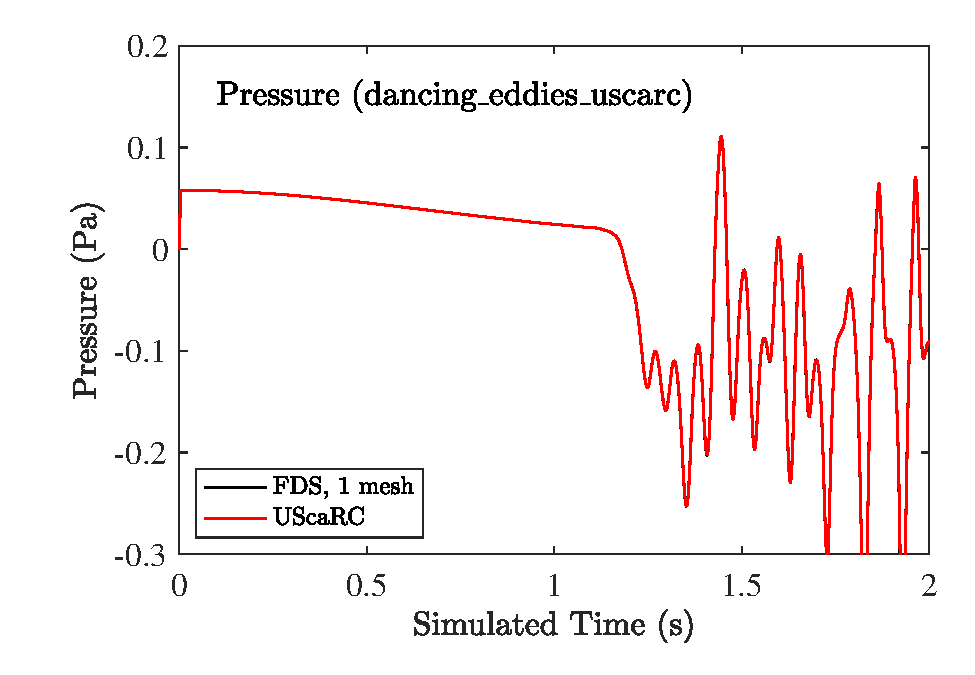
\includegraphics[width=3in]{\figPath/dancing_eddies_uscarc}
%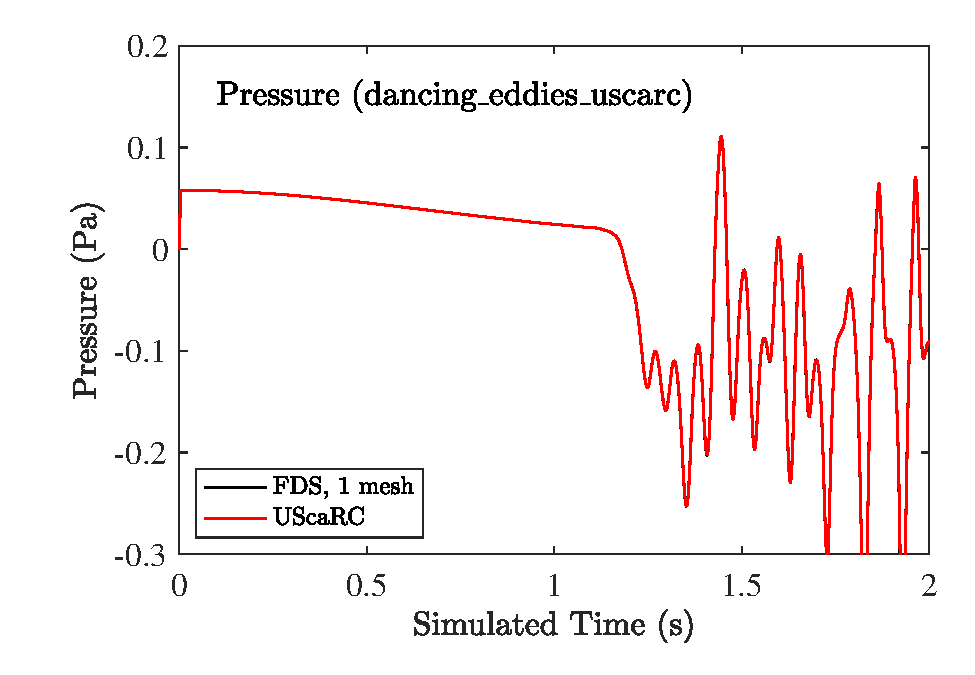
\includegraphics[width=3in]{\figPath/dancing_eddies_uscarc}   could be used ...
\end{center}
\caption[Results of the {\ct {\ct dancing\_eddies}} test cases]{Pressure traces of the default structured pressure solvers for the 4-mesh {\ct {\ct dancing\_eddies}} case compared to the single-mesh computation. (Left) \fftdefault{}. (Right) \scarcdefault{}.}
\label{FIG_scarc_dancing_eddies_pressure}
\end{figure}

\newpage
As already observed for \ffttight{} and \uglmat{} in the original test case, \scarctight{} and \uscarc{} show full agreement with the single mesh solution and are therefore not further illustrated graphically.
In contrast to \fftdefault{}, however, \scarcdefault{} already shows a good match for the coarse default tolerance as can be seen in Figure \ref{FIG_scarc_dancing_eddies_pressure}. 

Furthermore, Figure \ref{FIG_scarc_dancing_eddies_presite} displays a comparison of the required number of pressure iterations for the different solvers. The left plot shows a comparison for all solvers, the right plot omits \ffttight{} to give a zoomed view to the situation for the remaining solvers. 

\begin{figure}[ht]
\begin{center}
\includegraphics[width=3in]{\figPath/dancing_eddies/dancing_eddies_presite}
\includegraphics[width=3in]{\figPath/dancing_eddies/dancing_eddies_presite_zoom}
\end{center}
\caption[Results of different \scarc{} variants for the  {\ct {\ct dancing\_eddies}} test cases]{Comparison of the required number of pressure iterations. (Left) All solvers. (Right) Zoomed view to all solvers except of \ffttight{}.}
\label{FIG_scarc_dancing_eddies_presite}
\end{figure}

\fftdefault{} (cyan) needs 9 pressure iterations in maximum, but associated with the differences for the volume flow displayed in Figure \ref{FIG_scarc_dancing_eddies_pressure}. \ffttight{} (black) gives an accurate result, but requires averagely 24 iterations, occasionally even up to 120. 
In contrast, \scarcdefault{} (red) only needs a maximum of 2 iterations, but on average only 1, while already reaching a high approximation accuracy as seen for the pressure trace in the right plot of Figure \ref{FIG_scarc_dancing_eddies_pressure} above.
Thus, the requirements of \scarctight{} (magneta) are hardly more, it needs at most 4 and on average also only 1 iteration
to fulfil the finer tolerance.
By construction, \uglmat{} (blue) and \uscarc{} (green) are finished within exactly 1 iteration.
Please note again that the maximum and mean statistics were only performed after a certain initialization time of 0.1 s in order to exclude the large fluctuations at the beginning seen for the tight variants.

\subsubsection{Subdivision into 10 meshes ({\ct dancing\_eddies\_10mesh})}
To analyze the scalability of the various solvers, a subdivision into 10 instead of the previous 4 meshes is considered as well, see Figure \ref{FIG_scarc_dancing_eddies_ten}. Now, the same analysis is performed again.

\begin{figure}[ht]
\begin{center}
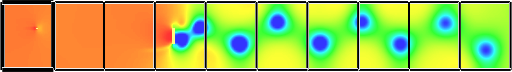
\includegraphics[width=0.9\textwidth]{\figPath/dancing_eddies_10mesh/dancing_eddies_10mesh_geometry}
\end{center}
\caption[Results of the {\ct {\ct dancing\_eddies}} test cases with 10 meshes]{Contour plot of the pressure for \uscarc{} after 2~s in case of a 10-mesh subdivision.}
\label{FIG_scarc_dancing_eddies_ten}
\end{figure}

Figure \ref{FIG_scarc_dancing_eddies_ten_convergence} gives an overview of the approximation quality of the different pressure solvers.
The lower-left plot therein shows that  \fftdefault{} (cyan) reaches the default tolerance  in an average of 3 and a maximum of 9 iterations.
However, as the top-left plot reveals, this isn't enough to capture the course of the pressure trace completely. The resulting oscillations are even more pronounced than for the 4-mesh case while the remaining solvers show full consistency again.
In particular, \ffttight{} (black) matches perfectly, but it also needs comprehensively more pressure iterations to fulfil the finer tolerance (averagely 28 iterations, but occasionally up to 99). %Once more, the initialization phase was not included in the statistical calculations.

\begin{figure}[ht]
\begin{center}
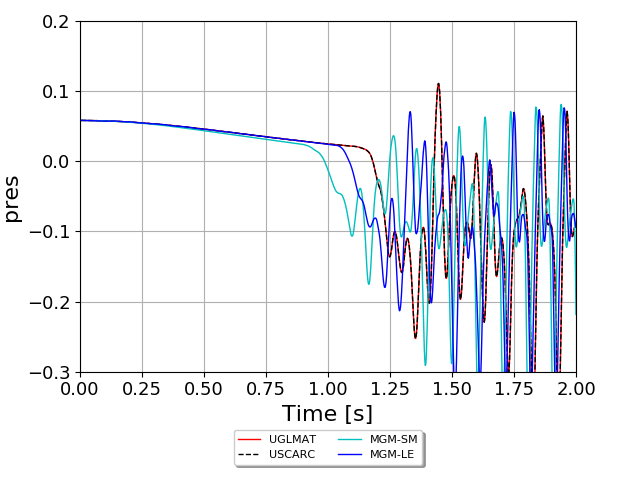
\includegraphics[width=3in]{\figPath/dancing_eddies_10mesh/dancing_eddies_pres}
\includegraphics[width=3in]{\figPath/dancing_eddies_10mesh/dancing_eddies_scarc}
\includegraphics[width=3in]{\figPath/dancing_eddies_10mesh/dancing_eddies_presite}
%\includegraphics[width=3in]{\figPath/dancing_eddies_10mesh/dancing_eddies_presite_zoom}
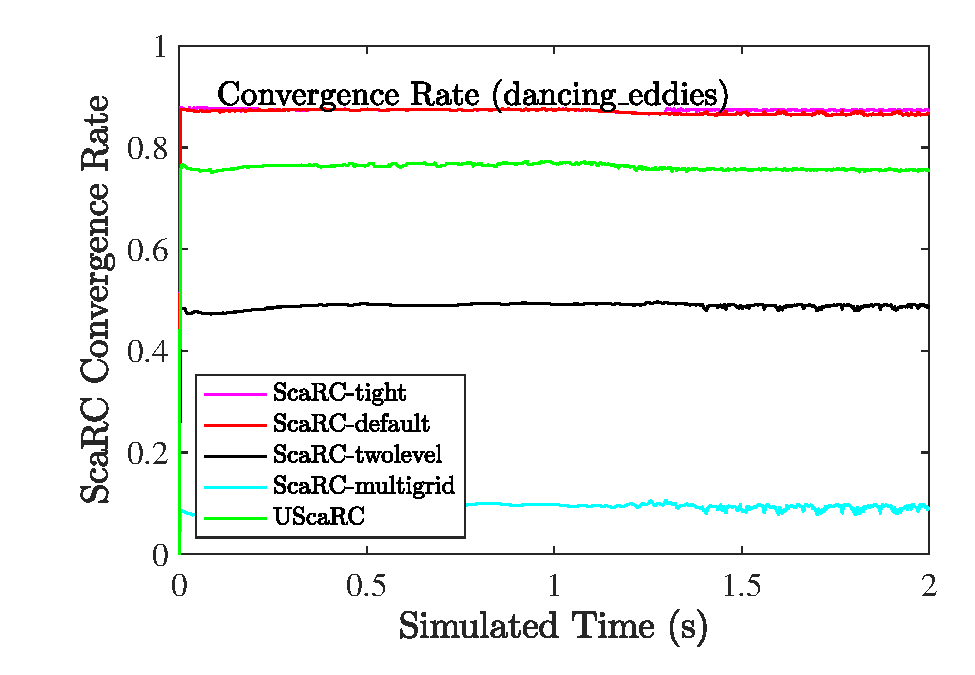
\includegraphics[width=3in]{\figPath/dancing_eddies_10mesh/dancing_eddies_scarc_rate}
\end{center}
\caption[Results for a 10-mesh computation of the {\ct {\ct dancing\_eddies}} case]{Results of different pressure solvers for a  {\ct {\ct dancing\_eddies}} test case subdivided into 10 meshes. (Top-left) Pressure traces of all solvers. (Top-right) Sole pressure trace of \scarcdefault{}.
(Bottom-left) Number of pressure iterations for all solvers.
(Bottom-right) Convergence rates of different \scarc{} variants. }
\label{FIG_scarc_dancing_eddies_ten_convergence}
\end{figure}

The top-right plot of Figure \ref{FIG_scarc_dancing_eddies_ten_convergence} proves that the 10-mesh \scarcdefault{} already gives a sufficiently good approximation of the pressure trace.
Furthermore, there is no big difference between \scarcdefault{} and \scarctight{}, both need only 1 iteration on average and not more than 2 or 4 at the maximum. Again, \uscarc{} and \uglmat{} match perfectly in 1 iteration.
Due to the increasingly transient nature of the flow, all solvers need more pressure iterations in the later course of the simulation, but it seems to stay within bounds for all.

Furthermore the bottom-right plot in Figure \ref{FIG_scarc_dancing_eddies_ten_convergence} displays the convergence rates of the different \scarc{} variants. 
Obviously, the additional use of a coarse grid level within \scarctwolevel{} almost leads to a halving of the convergence rate to 0.49, while the other CG-based variants lie in the range of a slow 0.8 or even worse. Especially for longer pipe-shaped domains like the one considered here, it can be very advantageous to use a coarse grid in order to spread at least a coarse average of the global information over the complete length of the domain. 

As expected, only the MG variant is out of the scope here in a positive sense and delivers a convergence rate of only 0.09 which, however, required some sensitive preliminary studies to adjust the optimal parameters. In this context, we refer again to the considerations on the evaluation of the overall performance at the end of Section \ref{SEC_SCARC_poisson_generalizations}.
 

A final look to the CPU-times in Figure \ref{FIG_scarc_dancing_eddies_cpu} shows that, 
despite the sometimes higher number of pressure iterations, that at least for the 4-mesh case \scarctight{} gives a smaller CPU time than \uscarc{} although its convergence rate is still worse. That's because
in case of structured \scarc{}, the locally regular grids allow the use of local FFT methods for preconditioning, which can be performed with highest performance. In case of unstructured \uscarc{},  local LU decompositions must be used instead.
Although these are also taken from an optimized program package, the Intel\textsuperscript{\textregistered} MKL library, they unfortunately prove to be slower than the local FFTs. Strategies to deal with these observations and to improve the situation are currently in work. 

In the 4-mesh case \uglmat{} performes best. But the situation changes for the 10-mesh case since the $LU$-decomposition  also suffers from increased communication effort for larger mesh numbers. Here the different \scarc{} variants are in the same range as \ffttight{}, while \uglmat{} and \scarcmultigrid{} are in the midfield 
The \scarctwolevel{} variant, despite its better convergence rate, needs the longest computing time and still requires computational improvement.
Basically, for the generalized structured \scarc{} variants there is still a
lot of room for further optimisation since they also can make use of local FFTs for smoothing which will be tested soon.



\begin{figure}[ht]
\begin{center}
\includegraphics[width=3in]{\figPath/dancing_eddies/dancing_eddies_all_cpu}
\includegraphics[width=3in]{\figPath/dancing_eddies_10mesh/dancing_eddies_all_cpu}
\end{center}
\caption[CPU times of different pressure solvers for the 4- and 10-mesh {\ct {\ct dancing\_eddies}} test cases]{CPU times of different pressure solvers for the 4- and 10-mesh {\ct {\ct dancing\_eddies}} test case}
\label{FIG_scarc_dancing_eddies_cpu}
\end{figure}

In summary, two important observations can be made:
%
For this special case, the domain decomposition seems to place greater demands on the pressure solver than the inner obstruction.
Thus, the worse convergence for \fftdefault{} compared to \scarcdefault{} (despite the same default tolerance) can be explained by the fact that the error influence observed in \fftdefault{} is essentially caused by the domain decomposition, but not by the inner obstruction. 
This doesn't hold true for \scarc{}
since all considered variants solve for the global pressure matrix and no longer produce velocity errors along the mesh interfaces. The remaining slight increase of pressure iterations is only related to the correction of the velocity errors along the internal obstruction which, in this special case, already works quite well for the default tolerance.  

In view of the small number of internal obstructions considered here, it does not really seem to be necessary to perform a tighter pressure iteration for structured \scarc{}, but the default velocity tolerance is already sufficient to reach a good approximation accuracy. 
Due to the mentioned runtime differences for the structured and unstructured preconditioners, there is no big advantage in taking the unstructured \uscarc{} in this case. The unstructured variant would only make sense if it achieved a substantially more accurate approximation along the inner obstruction (or the same in a comprehensibly shorter time), which is not the case here.
But this must not be understood as a general rule. As the {\ct duct\_flow} case \ref{SEC_SCARC_duct_flow} will show, the situation can be completely different if the influence of the internal obstructions is much larger than that of the domain decomposition.


% ======================================================================================
% duct_flow case
% ======================================================================================
\subsection{Flow through a duct ({\ct duct\_flow})}
\label{SEC_SCARC_duct_flow}

The next section follows the {\ct duct\_flow} case from the Pressure\_Solver verification directory which is defined on a cubic domain of side length 6.4~m. A subdivision into 8 meshes and a grid resolution of 0.2~m are used. 
With a speed of 1~m/s, air is pushed into a multi-angled duct of size 1 m$^2$ which meanders through the domain, as
illustrated in Figure \ref{FIG_scarc_duct_flow_flowfield}. 
Since there is no thermal expansion, the volume flow at the inlet and the outlet of the duct must be the same which provides a good basis test for the approximation quality of the different solvers. More information can be found in the FDS User's Guide\cite{McGrattan:2018:UG}.r


\begin{figure}[ht]
\centering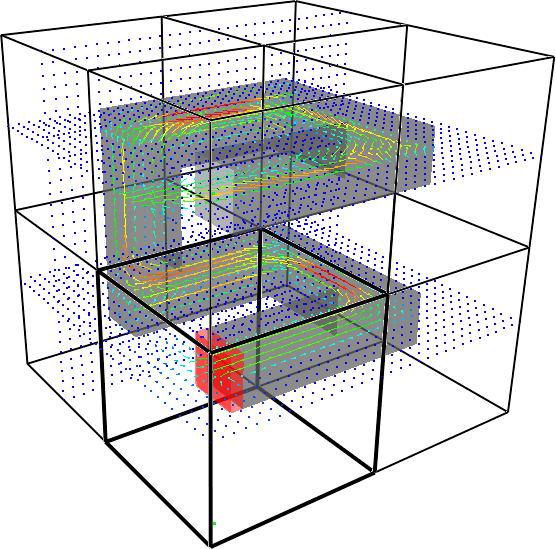
\includegraphics[width=3.0in]{\figPath/duct_flow/duct_flow_flowfield}
\caption{Flow field of the {\ct duct\_flow} case for a 8-mesh subdivision}
\label{FIG_scarc_duct_flow_flowfield}
\end{figure}

\newpage
By design, the flow is only limited to the inside of the duct and is forced to frequent changes of direction due to the numerous internal obstructions. This situation places particularly high demands on the structured pressure solvers to ensure a correct boundary approximation there. The subdivision of the domain into individual subdomains makes the situation even more difficult.

In order to classify both possible error influences, namely at inner obstructions and at mesh interfaces, the different pressure solvers introduced in Section \ref{SEC_SCARC_verification} are applied and compared. Unfortunately, the default structured solvers, \fftdefault{} and \scarcdefault{}, are not capable of providing sufficient accuracy along the internal obstructions and will be omitted subsequently. For the tight structured variants, \ffttight{} and \scarctight{}, a {\ct VELOCITY\_TOLERANCE} of 0.001~m/s is used along with {\ct MAX\_PRESSURE\_ITERATIONS} set to 1000. Furthermore, the unstructured solvers, \uglmat{} and \uscarc{},  are applied as well.
 
According to the original study the left plot in Figure \ref{FIG_scarc_duct_flow_volumeflow} compares the recorded volume flows at the in- and outflow while the right plot shows the number of required pressure iterations.
For both structured solvers, \ffttight{} and \scarctight{}, considerable differences between the in- and outflow get obvious. However, despite occasional larger outbreaks, \scarctight{} mostly requires less pressure iterations than \ffttight{}. This is based on the fact that \ffttight{} additionally has to correct the velocity field along inner boundaries, which is not the case for \scarctight{}. 

Nevertheless, it seems that for this case the main cause of errors can be traced back to the variety of inner obstructions. 
All in all, both structured variants do not really deliver satisfactory results here.
Instead, both unstructured solvers \uglmat{} and \uscarc{} provide exact matches for the outflow while needing exactly one pressure iteration.

\begin{figure}[ht]
\begin{center}
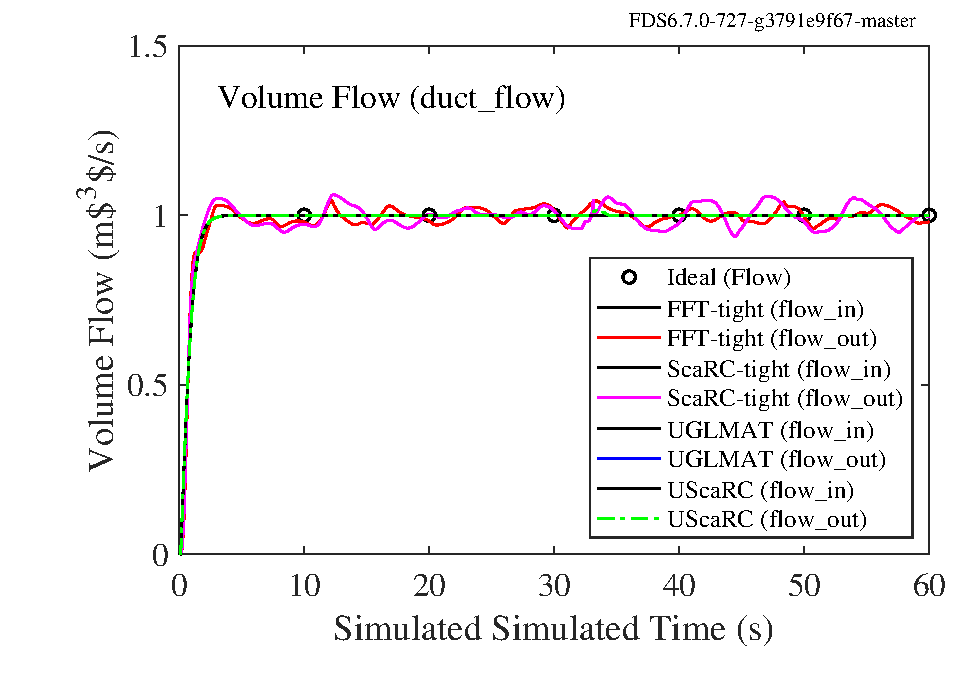
\includegraphics[width=3in]{\figPath/duct_flow/duct_flow_flowdiff}
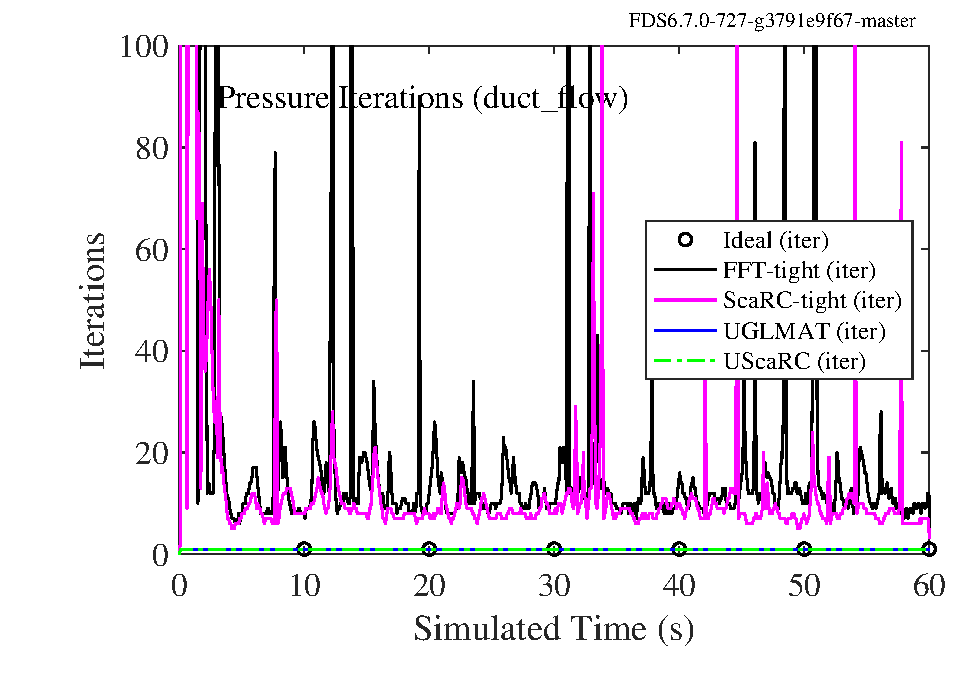
\includegraphics[width=3in]{\figPath/duct_flow/duct_flow_presite}
\end{center}
\caption[Results of the {\ct {\ct duct\_flow}} test case]{(Left) Volume flow into and out of a square duct. (Right) The number of pressure iterations as a function of time.}
\label{FIG_scarc_duct_flow_volumeflow}
\end{figure}

In contrast to the {\ct {\ct dancing\_eddies}} case, in which the application of the structured solvers was even more time-efficient, the unstructured solvers can play out their full potential for irregular grids here and deliver better results by far. 
This becomes especially clear in Figure \ref{FIG_scarc_duct_flow_velerror} which compares the 
velocity errors along the walls of the duct for the structured and the unstructured variants. 

\begin{figure}[ht]
\begin{center}
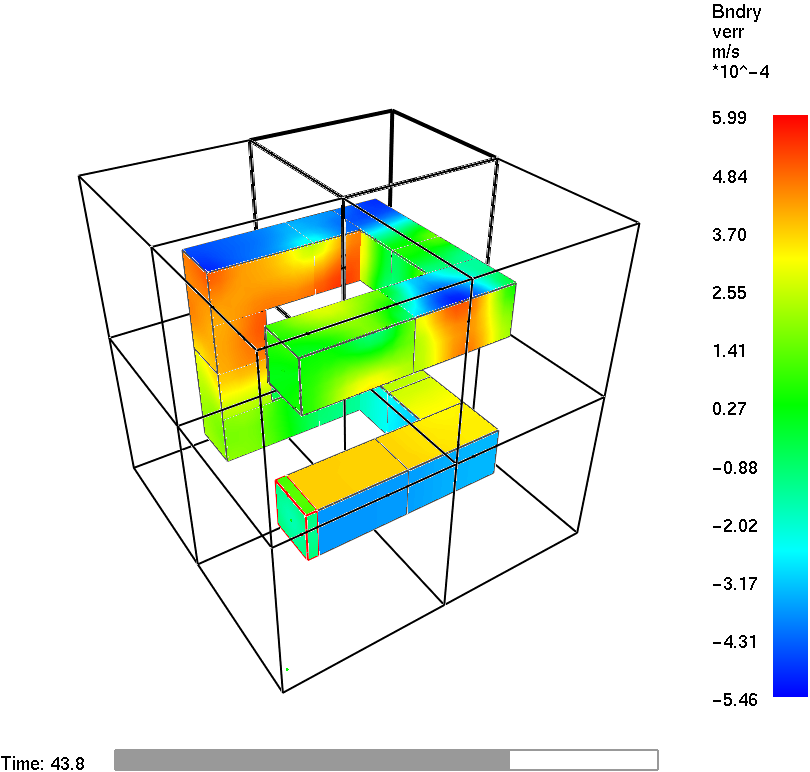
\includegraphics[width=3in]{\figPath/duct_flow/duct_flow_0364.png}
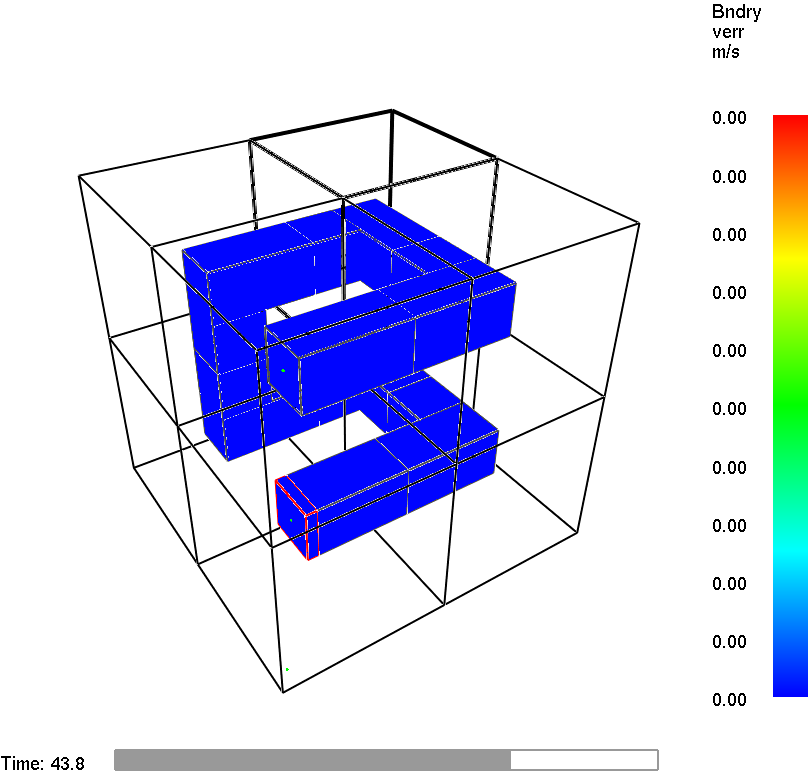
\includegraphics[width=3in]{\figPath/duct_flow/duct_flow_uscarc_0365.png}
\end{center}
\caption[Velocity error along internal obstructions in {\ct {\ct duct\_flow}} case]{Velocity error along internal obstructions in {\ct {\ct duct\_flow}} case. (Left) The error is in the range $10^{-3}$ for  \ffttight{} and \scarctight{} (Right) Machine precision is reached for \uglmat{} and \uscarc{}. }
\label{FIG_scarc_duct_flow_velerror}
\end{figure}

In the left plot a snapshot of \ffttight{} at $t=43.8$~s is shown. Despite the high number of pressure iterations there are obvious errors which can only be further reduced at disproportionately great expense. Although it requires slightly fewer pressure iterations, \scarctight{} shows a comparable picture as well.
The large number of obstructions and the associated flow dynamics make it extremely difficult here for the structured solvers to achieve a good approximation with moderate effort.
These troubles clearly dominate the additional negative effect of the domain decomposition in this case, which is why both structured solvers are equally affected.
By contrast, the right plot shows the corresponding snapshot of \uscarc{} which gives machine precision instead. The same zero-error picture can be obtained for \uglmat{} as well.


Finally, the memory requirements of the \uglmat{} solver are analyzed.
This solver has to build the global $LU$-decomposition of the Poisson matrix $A$ and store it in a distributed way over all meshes.
Table \ref{TAB_scarc_duct_flow_memory_needs} compares the number of non-zeros of $A$ with that of the corresponding triangular matrix $L$ for different grid refinements of the current case as measured within the solver.

\begin{table}[h]
\begin{center}
{
\begin{tabular}{|r|r|r|r|}
\hline
Cells         &   $NNZ(A)$     &        $NNZ(L)$ &  $NNZ(L)/NNZ(A)$   \\  \hline
  $32^3$   &      125,685      &        4,513,040 &  36    \hspace{0.4in}                       \\
  $64^3$   &   1,027,008      &      82,630,016 &  81    \hspace{0.4in}                        \\
  $128^3$ &   8,300,736      & 1,693,459,406 &  204   \hspace{0.4in}                        \\  \hline
\end{tabular}
}
\caption[Growing memory need of \uglmat{} in case of a grid refinement]{Growing memory need of \uglmat{} in case of a grid refinement from $32^3$ to $128^3$ cells; The number of non-zero entries of the Poisson matrix $NNZ(A)$ is compared to the corresponding number $NNZ(L)$ of the triangular matrix $L$}
\label{TAB_scarc_duct_flow_memory_needs}
\end{center}
\end{table}


For the calculations shown above a total grid resolution of $32^3$ cells was considered. In this case
the ratio of the non-zeros between $L$ and $A$ already amounts to 36. 
If the grid is further refined, however, it drastically raises up to a ratio of 204 in case of $128^3$ cells. For this finer resolution
the application of the $LU$-decomposition requires additional memory for the storage of
about 1.69 billions of double precision values. 
In view of realistically large problems with a significantly higher number of grid cells and submeshes, this `memory-hunger' can become an invincible constraint. Thus, on a computing platform with a given amount of storage more finely resolved problems can be considered with FFT and \scarc{} since both are much less memory intensive.

At this point it must be mentioned that \uscarc{},  as an unstructured solver, also uses local $LU$-decompositions, because the application of the local FFT is no longer possible.
However, these are only built in the scope of the individual meshes and do not act across the entire domain. Thus the associated increase of memory requirements seems to be acceptable or does at least not grow with increasing number of meshes.
But as already mentioned, for performance reasons, alternatives for the local $LU$-decompositions are being worked on anyway.


% ======================================================================================
% Periodic boundary conditions
% ======================================================================================
\subsection{Periodic Boundaries}
\label{SEC_SCARC_periodic_boundaries}

A number of test cases which are based on periodic boundaries can be found in the FDS Verification Guide~\cite{McGrattan:2018:VG}. Periodic boundary conditions are often used to evaluate the quality of a `pure' solver without the disturbing influence of boundary effects. Alternatively, they are also used to reduce the size of a computational domain for a problem with recurring patterns.

For single-mesh cases true periodic boundary conditions can be easily integrated into the Crayfishpak-based FFT solver. Unfortunately, this is not possible in the multi-mesh case. Here, matrix entries belonging to a periodic boundary cell are interpreted as Dirichlet entries for which the solution value is explicitly specified. Missing values are exchanged between the related `periodic neighbors' in the subdivision. While reasonable results can be achieved, this approach is not entirely correct and possibly leads to small errors in the solution. More information can be found in the corresponding section of the FDS User's Guide~\cite{McGrattan:2018:UG}.

In contrast to that, \scarc{} is able to apply true periodic boundary conditions also in the multi-mesh case. Instead of the Dirichlet-based matrix stencil used for the mesh-wise FFT solver, a true periodic matrix stencil is incorporated into the Poisson matrix. Again, the values for the missing `legs' 
%of the periodic stencils 
are correspondingly exchanged. 
To prevent the system from becoming indefinite, a corresponding {\it condensed system} is used. More detailed algorithmic information on this topic will follow.
To check the basic correctness of this procedure, some of the available periodic test cases in FDS were also performed with different \scarc{} variants und will be briefly summarized below.


\subsubsection{Analytical Solution to Navier-Stokes Equation ({\ct ns2d\_4mesh, ns2d\_16mesh})}

This series of test cases, from Verification/NS\_Analytical\_Solution, is concerned with the approximation of a given analytical solution for the 2D incompressible Navier-Stokes equations. 
%\begin{equation}
%\label{eqn_NS}
%\frac{\partial \mathbf{u}}{\partial t} + \mathbf{u} \cdot \nabla \mathbf{u} = - \nabla{p} + \nu \nabla^2 \mathbf{u} \,\mbox{,}
%\end{equation}
%
The basic geometry is a square of side length $L=2\pi$ with a uniform grid resolution of $\delta x = \delta z = L/N$ in each direction for which different resolutions $N =\{8,16,32,64\}$ are analyzed.  The resulting solutions are spatially periodic on the interval $2\pi$. Furthermore, the inviscid case $\nu=0$ and a viscous case $\nu=0.1$ are considered. In the inviscid case the solution happens to be also temporally periodic on $2\pi$.
Detailed information can be obtained in the corresponding section of the FDS Verification Guide~\cite{McGrattan:2018:VG}.

Several multi-mesh computations were performed with structured \scarcdefault{}.
According to the analysis in the FDS Verification Guide~\cite{McGrattan:2018:VG}, Figure \ref{FIG_scarc_ns_analytical_solution_uvel} shows the initial ($t=0$) and final ($t=2\pi$) state of the numerical solution 
for the grid resolution $N=64$ and a 16-mesh subdivision of the domain. 
Due to the temporal periodicity, the analytical solution requires both to be completely identical.
And in fact, 16-mesh \scarcdefault{} works correctly and remains in conformity with the analytical conditions.
This means in particular that the periodic boundary conditions are correctly integrated into the system of equations.
%
\begin{figure}[ht]
\begin{center}
%
\begin{minipage}{0.4\textwidth}
\begin{center}
$t=0.0~s$\\[1ex]
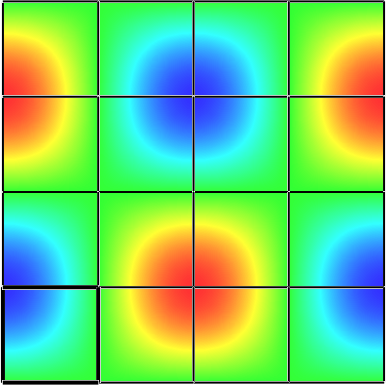
\includegraphics[height=2.0in]{\figPath/ns2d_16mesh/ns2d_16mesh_64_start.png}
\end{center}
\end{minipage}
\begin{minipage}{0.4\textwidth}
\begin{center}
$t=6.28~s$ \\[1ex]
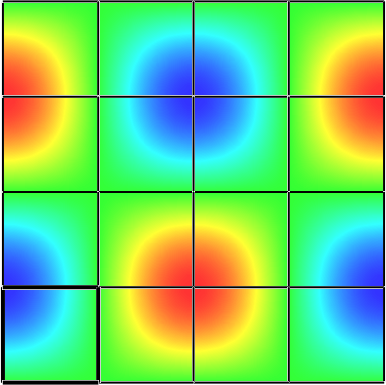
\includegraphics[height=2.0in]{\figPath/ns2d_16mesh/ns2d_16mesh_64_stop.png}
\end{center}
\end{minipage}
\begin{minipage}{0.1\textwidth}
\begin{center}
\quad $m/s$ \\[1ex]
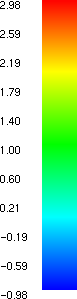
\includegraphics[height=2.0in]{\figPath/ns2d_16mesh/ns2d_16mesh_64_legend.png}
\end{center}
\end{minipage}
%
\end{center}
\caption[16-mesh \scarc{} computation of the {\ct NS\_Analytical\_Solution} case]{Identical initial and final state of the $u$-component of velocity for a 16-mesh \scarc{} computation of the {\ct NS\_Analytical\_Solution} case, showing that \scarc{} is able to treat periodic boundary conditions for multi-mesh cases, too.}
\label{FIG_scarc_ns_analytical_solution_uvel}
\end{figure}

In the further course of the original test it was shown that in the single-mesh case %considered there 
the advective and viscous terms are approximated with second-order accuracy. In line with this analysis the related cases are analyzed with 4-mesh \scarcdefault{} and
the corresponding results are displayed in Figure \ref{FIG_scarc_ns_analytical_solution_time}. 
As can be seen, with increasing grid refinement \scarc{} clearly converges to the analytical solution. Moreover, as shown in 
Figure \ref{FIG_scarc_ns_analytical_solution_rate} for both the inviscid and the viscous case, it also preservers the second order convergence rate of the original single-mesh scheme. 

\begin{figure}[!ht]
   \begin{tabular*}{\textwidth}{l@{\extracolsep{\fill}}r}
      \scalebox{1.0}{ 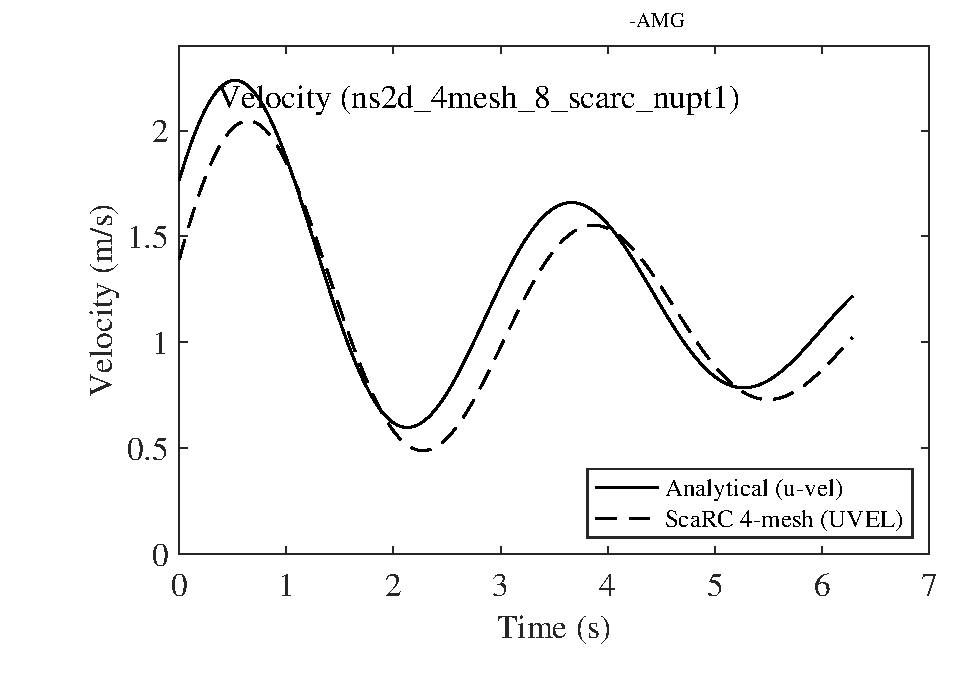
\includegraphics[height=2.2in]{\figPath/ns2d_4mesh/ns2d_4mesh_8_scarc_nupt1} } &
      \scalebox{1.0}{ 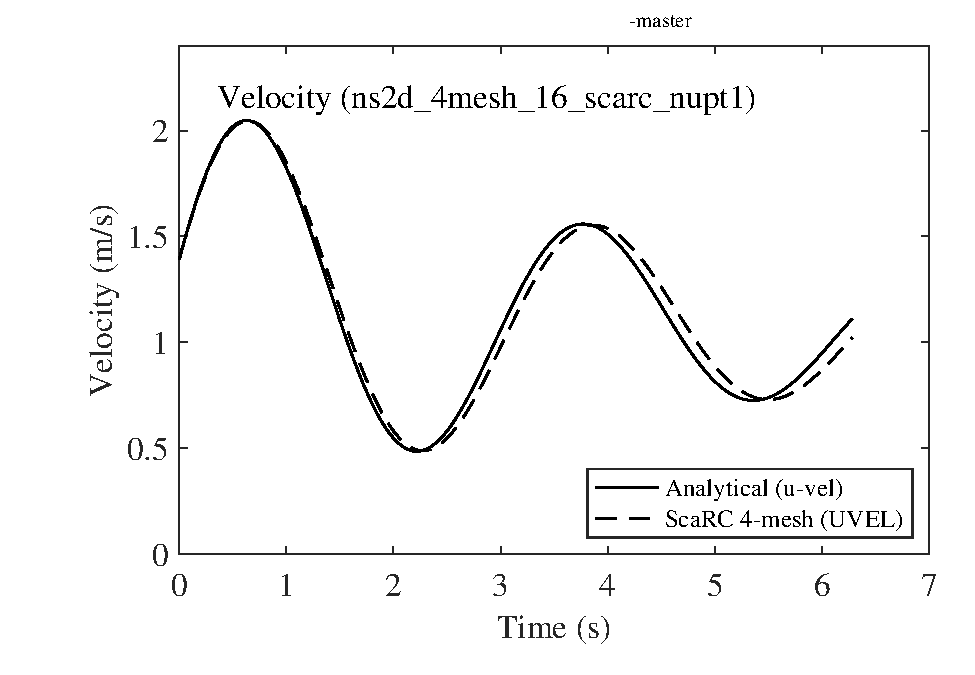
\includegraphics[height=2.2in]{\figPath/ns2d_4mesh/ns2d_4mesh_16_scarc_nupt1} } \\ 
      \scalebox{1.0}{ 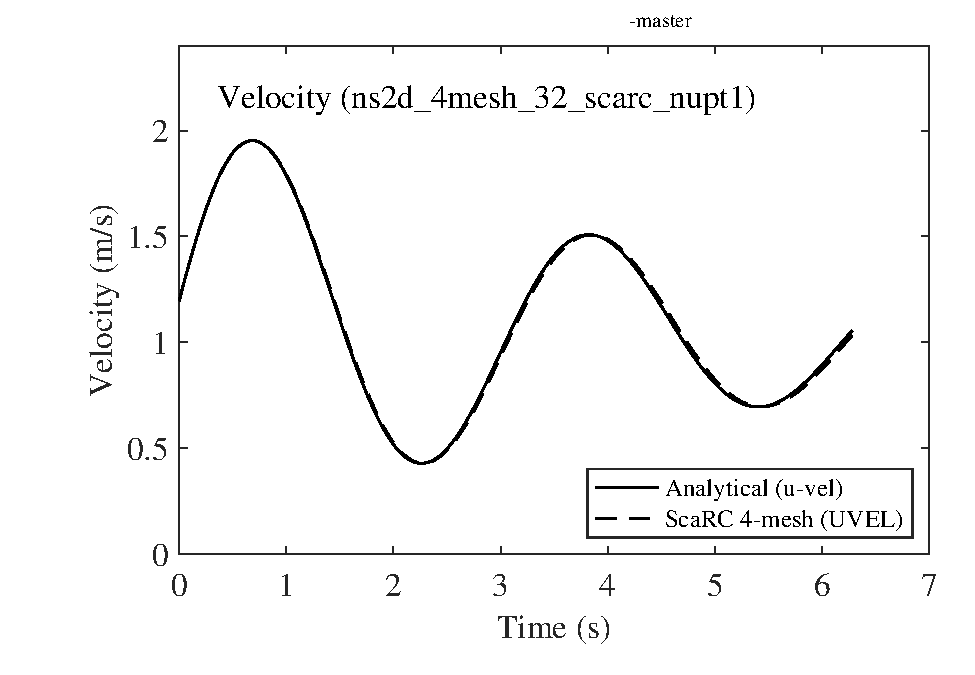
\includegraphics[height=2.2in]{\figPath/ns2d_4mesh/ns2d_4mesh_32_scarc_nupt1} } &
      \scalebox{1.0}{ 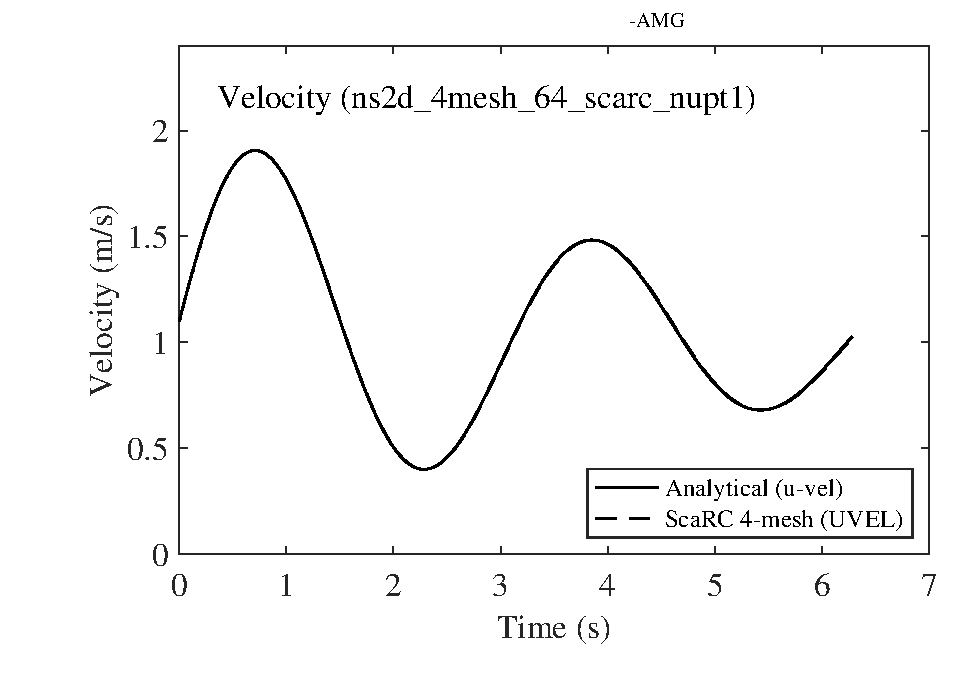
\includegraphics[height=2.2in]{\figPath/ns2d_4mesh/ns2d_4mesh_64_scarc_nupt1} }
   \end{tabular*}
   \caption[Velocity time history, qualitative convergence for a 4-mesh \scarc{}]{Time history of the $u$-component of velocity for the {\ct NS\_Analytical\_Solution} case with
$\delta x = L/N$ where $L = 2\pi$ m and $N = \{8,16,32,64\}$ for a 4-mesh \scarc{} computation, showing that the second-order convergence for the single-mesh case is preserved by 4-mesh \scarc{}.}
   \label{FIG_scarc_ns_analytical_solution_time}
\end{figure}


\begin{figure}[!ht]
   \begin{tabular*}{\textwidth}{l@{\extracolsep{\fill}}r}
      \scalebox{1}{ 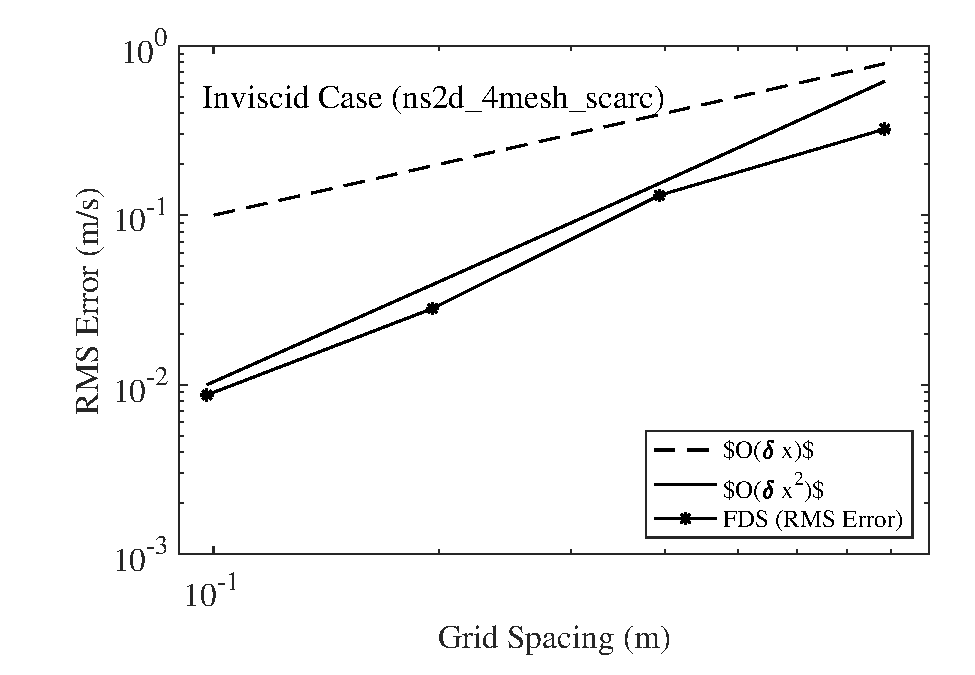
\includegraphics[height=2.2in]{\figPath/ns2d_4mesh/ns2d_4mesh_scarc_error} } &
      \scalebox{1}{ 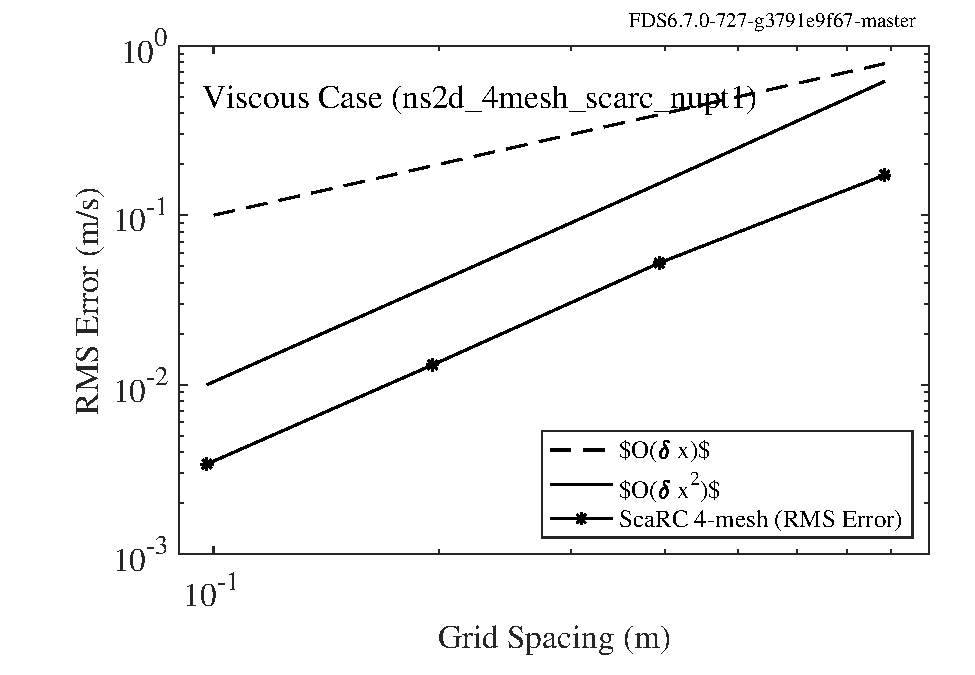
\includegraphics[height=2.2in]{\figPath/ns2d_4mesh/ns2d_4mesh_scarc_nupt1_error} }
   \end{tabular*}
   \caption[Navier-Stokes convergence study for 4-mesh \scarc{}]
   {Convergence rate for the $u$-component of velocity  for a 4-mesh \scarc{} computation with  $\nu = 0$ (Left) and  
   $\nu=0.1$ (Right) for the {\ct NS\_Analytical\_Solution} case.
   The dashed and solid lines serves as references for first- and second-order accuracy.
   The second order accuracy for the advective terms of the original single-mesh case is preserved by 4-mesh \scarc{}.}
\label{FIG_scarc_ns_analytical_solution_rate}
\end{figure}


%\begin{figure}[ht]
%\begin{center}
%\hspace{0.2in}$t=0.0$\hspace{0.76in}$t=1.57$\hspace{0.71in}$t=3.14$\hspace{0.71in}$t=4.71$\hspace{0.71in}$t=6.28$ \\[1ex]
%\includegraphics[width=1.1in]{\figPath/ns2d_4mesh/ns2d_4mesh_64_1.png}\hspace{0.1in}
%\includegraphics[width=1.1in]{\figPath/ns2d_4mesh/ns2d_4mesh_64_2.png}\hspace{0.1in}
%\includegraphics[width=1.1in]{\figPath/ns2d_4mesh/ns2d_4mesh_64_3.png}\hspace{0.1in}
%\includegraphics[width=1.1in]{\figPath/ns2d_4mesh/ns2d_4mesh_64_4.png}\hspace{0.1in}
%\includegraphics[width=1.1in]{\figPath/ns2d_4mesh/ns2d_4mesh_64_5.png}
%\end{center}
%\caption[Results of different \scarc{} variants for the  {\ct NS\_Analytical\_Solution} case]{ ??}
%\label{FIG_scarc_ns_analytical_solution}
%\end{figure}

%\begin{figure}[ht]
%\begin{center}
%\includegraphics[width=3in]{\figPath/ns2d_4mesh_64_scarc_nupt1.pdf}
%\includegraphics[width=3in]{\figPath/ns2d_scarc_nupt1_error.pdf}
%\includegraphics[width=3in]{\figPath/ns2d_scarc_error.pdf}
%\end{center}
%\caption[Results of different \scarc{} variants for the  {\ct NS\_Analytical\_Solution} case]{ ??}
%\label{FIG_scarc_ns_analytical_solution}
%\end{figure}

\subsubsection{Variable-Density Manufactures Solution ({\ct shunn3\_16mesh})}

The {\ct shunn3} test case from Verification/Scalar\_Analytical\_Solution is intended to prove the second order accuracy of the FDS time-stepping scheme. It is based on a manufactured sinusoidal solution which diagonally translates across a square-shaped domain of side length 2. The solution is spatially periodic in this domain and has a time period of 1~s. 
Different grid resolutions of  $N = \{32, 64, 128, 256, 512\}$ cells per direction were considered there. 
The settings for this case are very complex and can be read in more detail in the FDS Verification Guide~\cite{McGrattan:2018:VG}.

As before, \scarc{} was applied for different subdivisions of this case into 4 and 16 meshes.
Exemplary, the evolution of the density $\rho$, the mixture fraction $Z$ and the u-velocity 
for the grid resolution of $256^2$ were shown in Figure \ref{FIG_scarc_shunn3} for a corresponding 16-mesh \scarc{} computation.
Obviously, the periodicity of the analytical solutions is completely preserved and there is no recognizable difference to the single mesh approximation, which in turn proves the correct handling of periodic boundary values for multi-mesh decompositions by \scarc{}.
 
\begin{figure}[ht]
\centering
\input{\utilPath/colormap.txt}
% density
\begin{tikzpicture}[scale=1]
\footnotesize
\begin{axis}[
    width=0.95\linewidth,
    axis equal image,
    enlargelimits=false,
    axis x line=none,
    axis y line=none,
    colorbar,
    colormap name=fds,
    point meta min=1, point meta max=5,
    colorbar style={
        title={$\rho$, \si{kg/m^3}},
        at={(1.02,0.0)}, % Coordinate system relative to the main axis. (1,1) is upper right corner of main axis.
        anchor=south west,
        height=\pgfkeysvalueof{/pgfplots/parent axis height}, % Scale the colorbar relative to the main axis
        /pgf/number format/.cd, % Change the key directory to /pgf/number format
        fixed, fixed zerofill, precision=1,
        /tikz/.cd  % Change back to the normal key directory
    }
    	]
	\addplot graphics [xmin=0.00, xmax=1.00, ymin=0, ymax=1] {\figPath/shunn3/density/shunn3_16mesh_256_scarc_p0000};
	\addplot graphics [xmin=1.10, xmax=2.10, ymin=0, ymax=1] {\figPath/shunn3/density/shunn3_16mesh_256_scarc_p0041};
	\addplot graphics [xmin=2.20, xmax=3.20, ymin=0, ymax=1] {\figPath/shunn3/density/shunn3_16mesh_256_scarc_p0086};
	\addplot graphics [xmin=3.30, xmax=4.30, ymin=0, ymax=1] {\figPath/shunn3/density/shunn3_16mesh_256_scarc_p0131};
\end{axis}
\draw (1.75,3.78) node {$t=0$ s};
\draw (5.25,3.78) node {$t=0.125$ s};
\draw (8.8,3.78) node {$t=0.250$ s};
\draw (12.5,3.78) node {$t=0.375$ s};
\end{tikzpicture}

% mixture fraction
\begin{tikzpicture}[scale=1]
\footnotesize
\begin{axis}[
    width=0.95\linewidth,
    axis equal image,
    enlargelimits=false,
    axis x line=none,
    axis y line=none,
    colorbar,
    point meta min=0, point meta max=1,
    colormap name=fds,
    colorbar style={
        title={$Z$},
        at={(1.02,0.0)}, % Coordinate system relative to the main axis. (1,1) is upper right corner of main axis.
        anchor=south west,
        height=\pgfkeysvalueof{/pgfplots/parent axis height}, % Scale the colorbar relative to the main axis
        /pgf/number format/.cd, % Change the key directory to /pgf/number format
        fixed, fixed zerofill, precision=1,
        /tikz/.cd  % Change back to the normal key directory
    }
    	]
	\addplot graphics [xmin=0.00, xmax=1.00, ymin=0, ymax=1] {\figPath/shunn3/Z/shunn3_16mesh_256_scarc_p0000};
	\addplot graphics [xmin=1.10, xmax=2.10, ymin=0, ymax=1] {\figPath/shunn3/Z/shunn3_16mesh_256_scarc_p0041};
	\addplot graphics [xmin=2.20, xmax=3.20, ymin=0, ymax=1] {\figPath/shunn3/Z/shunn3_16mesh_256_scarc_p0086};
	\addplot graphics [xmin=3.30, xmax=4.30, ymin=0, ymax=1] {\figPath/shunn3/Z/shunn3_16mesh_256_scarc_p0131};
\end{axis}
\end{tikzpicture}

% uvelocity
\begin{tikzpicture}[scale=1]
\footnotesize
\begin{axis}[
    width=0.95\linewidth,
    axis equal image,
    enlargelimits=false,
    axis x line=none,
    axis y line=none,
    colorbar,
    point meta min=0.2, point meta max=0.8,
    colormap name=fds,
    colorbar style={
        title={$u$, m/s},
        at={(1.02,0.0)}, % Coordinate system relative to the main axis. (1,1) is upper right corner of main axis.
        anchor=south west,
        height=\pgfkeysvalueof{/pgfplots/parent axis height}, % Scale the colorbar relative to the main axis
        /pgf/number format/.cd, % Change the key directory to /pgf/number format
        fixed, fixed zerofill, precision=1,
        /tikz/.cd  % Change back to the normal key directory
    }
    	]
	\addplot graphics [xmin=0.00, xmax=1.00, ymin=0, ymax=1] {\figPath/shunn3/uvel/shunn3_16mesh_256_scarc_p0000};
	\addplot graphics [xmin=1.10, xmax=2.10, ymin=0, ymax=1] {\figPath/shunn3/uvel/shunn3_16mesh_256_scarc_p0041};
	\addplot graphics [xmin=2.20, xmax=3.20, ymin=0, ymax=1] {\figPath/shunn3/uvel/shunn3_16mesh_256_scarc_p0086};
	\addplot graphics [xmin=3.30, xmax=4.30, ymin=0, ymax=1] {\figPath/shunn3/uvel/shunn3_16mesh_256_scarc_p0131};
\end{axis}
\end{tikzpicture}

\caption[Evolution of the variable-density manufactured solution for a 16-mesh \scarc{} computation]{Evolution of the variable-density manufactured solution for a 16-mesh \scarc{} computation for the {\ct shunn3} case.  From top to bottom, the images show density, $\rho$, mixture fraction, $Z$, and the $u$-velocity component from the $256^2$ simulation at the specified times. The parallel computation by \scarc{} clearly preserves the periodicity of the analytical solution.}
\label{FIG_scarc_shunn3}
\end{figure}


%\begin{figure}[ht]
%\begin{center}
%\includegraphics[width=3in]{\figPath/shunn_4mesh_512_scarc_mms_convergence.pdf}
%\includegraphics[width=3in]{\figPath/shunn_16mesh_512_scarc_mms_convergence.pdf}
%\includegraphics[width=3in]{\figPath/shunn3.png}%
%\end{center}
%\caption[Results of different \scarc{} variants for the  {\ct shunn3} case]{ ??}
%\label{FIG_scarc_shunn3}
%\end{figure}


\subsubsection{Ribbed Square Duct Flow ({\ct ribbed\_channel\_4mesh})}

In the previous two cases, periodic boundary conditions were applied to the entire boundary of the computational domain. The situation is different, however, if there is a mixture of Neumann and periodic boundary conditions, since here only the periodic boundary values have to be communicated between the corresponding partners, while those for the Neumann components are set according to the boundary specifications of the case.

\newpage
\scarc{} is able to handle these components individually. For the Neumann parts of the boundary, corresponding Neumann matrix stencils are integrated into the system with according settings of the right hand side. For the periodic parts the corresponding periodic stencils are used.
As long as there are no additional Dirichlet components on the boundary, the condensed system must be used again
in order to avoid that the matrix becomes indefinite. 

Figure \ref{FIG_scarc_ribbed_channel} gives an example where periodic boundary conditions are used at
{\ct XMIN} and {\ct XMAX} while Neumann boundary conditions are used elsewhere which is related to the
Turbulence/ribbed\_channel test case.
More details can be found in the FDS Verification Guide \cite{McGrattan:2018:VG}.
Due to the large internal obstruction the unstructured \uscarc{} solver based on a 4-mesh subdivision was used. Evidently, the original flow pattern is matched again. 

\begin{figure}[ht]
\centering
\includegraphics[width=.8\textwidth]{\figPath/ribbed_channel/ribbed_channel_flow.png}
\caption[4-mesh \scarc{} computation for the {\ct ribbed\_channel} test case]{Mean velocity vectors colored by velocity magnitude (red is 2 m/s) for the ribbed square duct case with $h/\delta x = 8$ for a 4-mesh \uscarc{} computation for the {\ct ribbed\_channel} case.}
\label{FIG_scarc_ribbed_channel}
\end{figure}

\begin{figure}[ht]
\centering
   \begin{tabular*}{\textwidth}{l@{\extracolsep{\fill}}r}
      \includegraphics[height=2.2in]{\figPath/ribbed_channel/ribbed_channel_u_strm_uscarc} &
      \includegraphics[height=2.2in]{\figPath/ribbed_channel/ribbed_channel_u_prof_uscarc} \\
      \includegraphics[height=2.2in]{\figPath/ribbed_channel/ribbed_channel_urms_strm_uscarc} &
      \includegraphics[height=2.2in]{\figPath/ribbed_channel/ribbed_channel_urms_prof_uscarc} \\
   \end{tabular*}
   \caption[Mean and RMS velocity profiles for ribbed square duct flow in case of a 4-mesh \uscarc{} computation]{\label{fig_ribbed_channel} Mean and RMS velocity profiles for ribbed square duct flow in case of a 4-mesh \uscarc{} computation for the {\ct ribbed\_channel} case.}
\label{FIG_scarc_ribbed_channel_devices}
\end{figure}



This case aimed to predict the mean recirculation patterns on the windward and leeward side of the rib. To this end line devices were used at the floor and at the center of the duct. The corresponding measurements for the 4-mesh \uscarc{} computation are summarized in Figure \ref{FIG_scarc_ribbed_channel_devices}. Note, that in comparison to the original test case the cases for the finest case $h/\delta x = 16$ are still missing due to their large complexity and will be handled later.
%
In summary, these plots are in qualitative accordance with the original single-mesh values  
which again proves the basic correctness of the periodic boundary treatment and the parallel processing in \scarc{}.



